\section{Experiments}\label{eval}
We start by presenting two end-to-end scenarios based on a dataset of movies from IMDB and a dataset of medical donations from ProPublica.
These scenarios have real data and real errors, and we describe how these errors can affect statistical modeling problems.
Next, we evaluate a how dirty data may affect Machine Learning ``pipelines'' in an image classification example where we corrupted certain images.
Then, we evaluate each of the components of \sys on standard Machine Learning benchmarks (Tax Record Classification, EEG anomaly detection) with synthetic errors.

\subsection{Setup}
We compare \sys to alternative solutions along two primary axes: the sampling procedure to pick the next set of records to clean, and the model update procedure to incorporate the cleaned sample.
All of the compared approaches clean the same amount of data, and we evaluate the accuracy of the approaches as a function of the amount of data examined; defined as the number of evaluations of the user-specified $C(\dot)$ (cleaner) on a record whether or not the record is actually dirty.

\vspace{0.25em}
\noindent\textbf{Naive-Mix (NM): } In each iteration, Naive-Mix  draws a random sample, merges the cleaned sample back into the dataset, and re-trains over the entire dataset.

\vspace{0.25em}
\noindent\textbf{Naive-Sampling (NS): } In contrast to Naive-Mix, Naive-Sampling only re-trains over the set of records that have been cleaned so far.

\vspace{0.25em}
\noindent\textbf{Active Learning (AL): }
The samples are picked using Active Learning (more precisely, Uncertainty Sampling~\cite{settles2010active}), and the model is re-trained over the set of records cleaned so far.

\vspace{0.25em}
\noindent\textbf{Oracle (O): } Oracle has complete access to the ground truth, and in each iteration, selects samples that maximize the expected convergence rate.  It uses \sys's model update procedure.  

\begin{figure*}[t]
\centering
 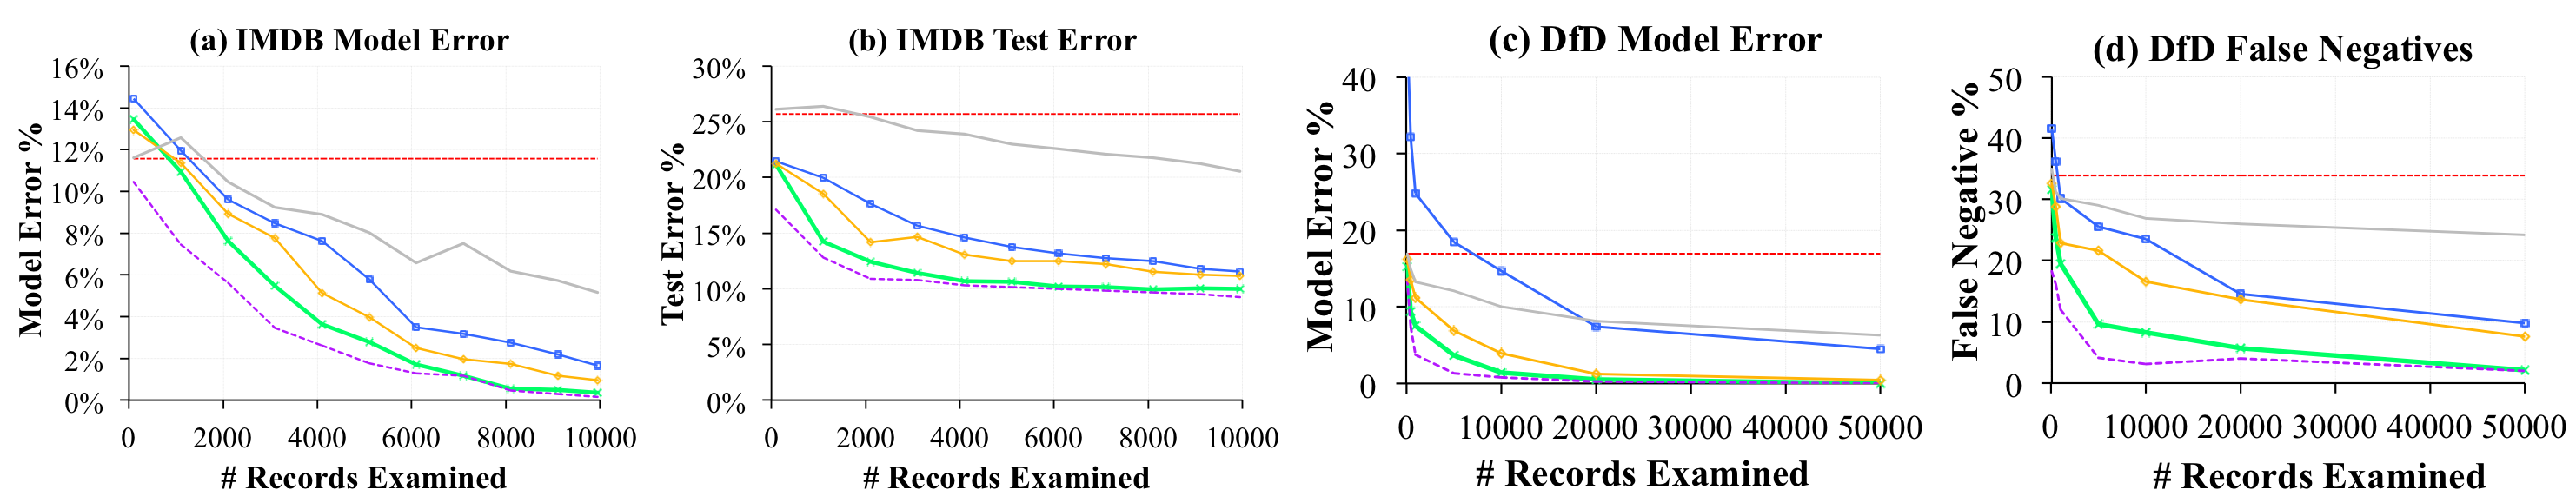
\includegraphics[width=\textwidth]{exp/real-experiments-full.png}
 
\includegraphics[width=0.6\columnwidth]{exp/legend-real.png}\vspace{-1em}
 \caption{(a) We plot the relative model error as a function of the number of records cleaned for each of the alternatives on the IMDB content tagging task. \sys results in the fastest convergence. (b) Faster convergence translates into improved test accuracy. On a holdout set of 20\%, \sys is more accurate than the alternatives. (c) We evaluate \sys on the Dollars For Docs fraud detection task and find similar results, where \sys converges faster than the alternatives. (d) \sys improves the false negative rate (detection error) of the classifier resulting in an improved fraud detector. \label{real}}\vspace{-1.5em}
\end{figure*}

\subsection{Real Scenarios}\label{real-errors}
We now describe two data analyst classification scenarios based on popular industry use cases reported in the Apache Spark user survey~\cite{sparksurvey} --- these experiments are run with real data and real corruption.
The first is a content tagging problem to categorize movies from plot descriptions; 
the second is a fraud detection problem to  determine whether a medical donation is suspicious.
Both of the datasets are plagued by systematic errors that affect the classification accuracy by $10-35\%$.
One indication of the systematic nature of the data error is that errors disproportionately affect one class rather than another.
We simulate the analyst's cleaning procedure by looking up the cleaned value in the dataset that we cleaned beforehand.
See~\cite{activecleanarxiv} for constraints, errors, and cleaning methodology, as well as an additional regression scenario.

%\reminder{Can I propose using "Records Examined" as the x-axes instead of "records cleaned"?}

\subsubsection{Movie Prediction (Movie)}\label{imdb}
The first scenario uses two movie datasets from IMDB \footnote{\tiny \url{ftp://ftp.fu-berlin.de/pub/misc/movies/database/}} and Yahoo that was published~\footnote{\tiny \url{http://webscope.sandbox.yahoo.com/catalog.php?datatype=r}}.
Each movie has a title, a short 1-2 paragraph plot description, and a list of categories, and the goal is to train a model to predict whether a movie is a ``Horror'' or ``Comedy'' from the description and title.  
The text data was featurized using a TFIDF model.

The IMDB dataset is larger (486,298), but much dirtier because it was collected from a web scraper.  
This data is user-contributed, and the category list is very dirty, with redundant and possibly conflicting tags (e.g., ``Kids'' and ``Horror'' for the same movie).  
Also, the plot and title text may have errors from the scraping procedure (e.g., ``results fr\^Celf, the'').
In contrast, the smaller (106,959 movies) Yahoo dataset is much cleaner, and nearly all of the movies are found in the IMDB dataset.
Thus, we used this as a cleaner reference dataset and performed simple entity resolution to match movies together, and imported the Yahoo dataset's categories to the IMDB dataset when possible.
For the movies that did not match, we appended the records to the IMDB dataset.
Finally, we filtered the dataset for movies whose category lists included ``Horror'' or ``Comedy''

% The first scenario explores a dataset of movie descriptions scrapped from the Internet Movie Database (IMDB)\footnote{\url{ftp://ftp.fu-berlin.de/pub/misc/movies/database/}}. 
% Each movie has a title, a 1-2 paragraph plot description, and a list of categories.
% We want to train a model that predicts whether a movie is a ``Horror'' movie or a ``Comedy'' from the plot description and the title.
% These textual attributes are featurized using a TFIDF model and stop words are removed. 
% 
% However, since much of this data is user contributed, the category list of the movies is often very dirty with redundant and sometimes conflicting tags (e.g., ``Kids and Family'' and ``Horror''). 
% Furthermore, the dataset was scrapped in HTML and then encoded in Markdown leaving a number of artifacts of parsing in the plot descriptions (e.g., ``results fr\^Celf, the'').
% Fortunately, we were able to find a much smaller but cleaner dataset from Yahoo of 106959 movies, almost all of which were contained in the IMDB dataset.
% Using this cleaner reference dataset, we matched titles and imported categories when possible.
% We also appended the cleaner plot descriptions from Yahoo to the IMDB descriptions when available.
% The clean dataset had about 10\% less examples than the dirty dataset since some movies were marked as neither  ``Horror'' or ``Comedy''.

Figure \ref{real}a plots the distance between the current and cleaned model parameters (model error) versus the number of $C(\dot)$ calls.  
%as more records are cleaned. 
The purple bottom curve is the Oracle approach, and we find that \sys reduces the model error the fastest, and is the only method that converges to the Oracle performance.
Figure~\ref{real}b directly shows how \sys rapidly reduces the test error --- after 2000 records, \sys's test error is within 0.02 of the fully cleaned model.
\sys provides superior convergence for several reasons.
First, the update algorithm can incorporate both the raw data as well as the smaller set of cleaned records.
On the other hand, the difference between Naive-Sampling and Naive-Mix in Figure~\ref{real}b highlights the effects of only using the cleaned data or combining clean and dirty datasets.
\sys selects records that are both more likely to by dirty (Section \ref{det}) and will most improve the model (Section \ref{dist-samp}).
This is illustrated in \sys's faster convergence curve in the first 2000 cleaned records.
The key reason for these positive results is the presence of systematic bias in the dataset as horror movies are more likely to be erroneously tagged.
Cleaning the dataset improved the test error for horror movies from 29 to 74\%.

% We find that \sys converges faster than those trained with the alternatives.
% The reasons for this include: (1) \sys samples more data that is likely to be dirty, and (2) \sys selects data that is most valuable to the model.
% This improvement in model convergence translates into large improvements in the accuracy of the model on a holdout set Figure \ref{real}b.
% Figure \ref{real}b illustrates two points: dirty data significantly affects the quality of the model (25\% misclassification rate) and a relatively small amount of data cleaning can greatly improve the quality of the model with the appropriate update techniques.
% For 2000 records cleaned, \sys is within 2\% of the accuracy of the model if the data were fully cleaned.
% On the other hand, for the same amount of cleaning, the ``Re-training'' approach hasn't improved the model. 

% One of the reasons for this positive result is the significant systematic bias in the errors. Horror movies were more likely to be erroneously tagged. 
% On the dirty dataset, the prediction precision of the model for Horror movies was only 29\%.
% This improved to 74\% after data cleaning.

\subsubsection{Dollars For Docs (DfD)}\label{exp:dfd}
The second scenario explores ProPublica's Dollars for Docs dataset described in Section\ref{s:usecase}.
The application featurizes the 5 text attributes using bag-of-words, and predicts the status of medical donations using a binary SVM.
Figure~\ref{real}c again shows that \sys outperforms the other cleaning approaches.
For instance, \sys requires 40,000 fewer calls to $C(\dot)$ in order to reduce the model error by $75\%$ as compared to the initial dirty model,
and exhibits nearly an order of magnitude smaller model error than either of the naive approaches after only 10,000 calls to $C(\dot)$.

Figure~\ref{real}d reports the detection error or false negative \% (percentage of disallowed research contributions that the model misses) rather than the overall test error because the former was the focus of the investigation.  The dirty and fully cleaned models have respectively a 34\% and 3\% detection error.
Due to the systematic bias in the data errors (explained in Section \ref{s:usecase}), \sys is able to identify the dirty records and
reduce the detection error to 8\% after 10,000 $C(\dot)$ calls, which is much faster than the alternatives.

Overall, we found that systematic errors are indeed present in real-world datasets, and that \sys can effectively identify and exploit this bias
to more quickly converge to the true clean model as compared to the naive or active learning approaches.  
In fact, we found that the commonly used retraining approach (Naive-Mix) was almost completely ineffective as compared to other model update techniques.
Thus, the further experiments focus on the other algorithms, and we discuss the difficulties of naively mixing dirty and clean data in Section~\ref{exp:rtr}.

% The dataset has 240,089 records with 5 textual attributes and one numerical attribute.
% The dataset is featurized with bag-of-words featurization model for the textual attributes which resulted in a 2021 dimensional feature vector, and a binary SVM is used to classify the status of the medical donations.
% Figure \ref{real}c shows that \sys converges faster than Active Learning and SampleClean.
% To achieve a 4\% relative error (i.e., a 75\% error reduction from the dirty model), \sys cleans 40000 fewer records than Active Learning.
% Also, for 10000 records cleaned, \sys has nearly an order of magnitude smaller error than SampleClean.

% Figure \ref{real}d shows the detection rate (fraction of disallowed research contributions identified) of the classifier as a function of the number of records cleaned. 
% On the dirty data, we can only correctly classify 66\% of the suspected examples (88\% overall accuracy due to a class imbalance).
% On the cleaned data, this classifier is nearly perfect with a 97\% true positive rate (98\% overall accuracy).
% \sys converges to the cleaned accuracy faster than the alternatives with a classifier of 92\% true positive rate for only 10000 records cleaned.
% These numbers also indicate the significant systematic bias where positive examples are more likely to be corrupted.

% In short, these two scenarios illustrate the value of \sys on real datasets both of which contain significant systematic biases.
% \sys demonstrates increased accuracy for the same amount of records cleaned compared the alternatives.
% Across all of our experimental datasets, we found that the retraining approach gave poor results in addition to the correctness problems discussed in the introduction.
% For this reason, in future comparisons, we exclude retraining but discuss this in Section \ref{exp:rtr}.

\begin{figure}[t]
\centering
 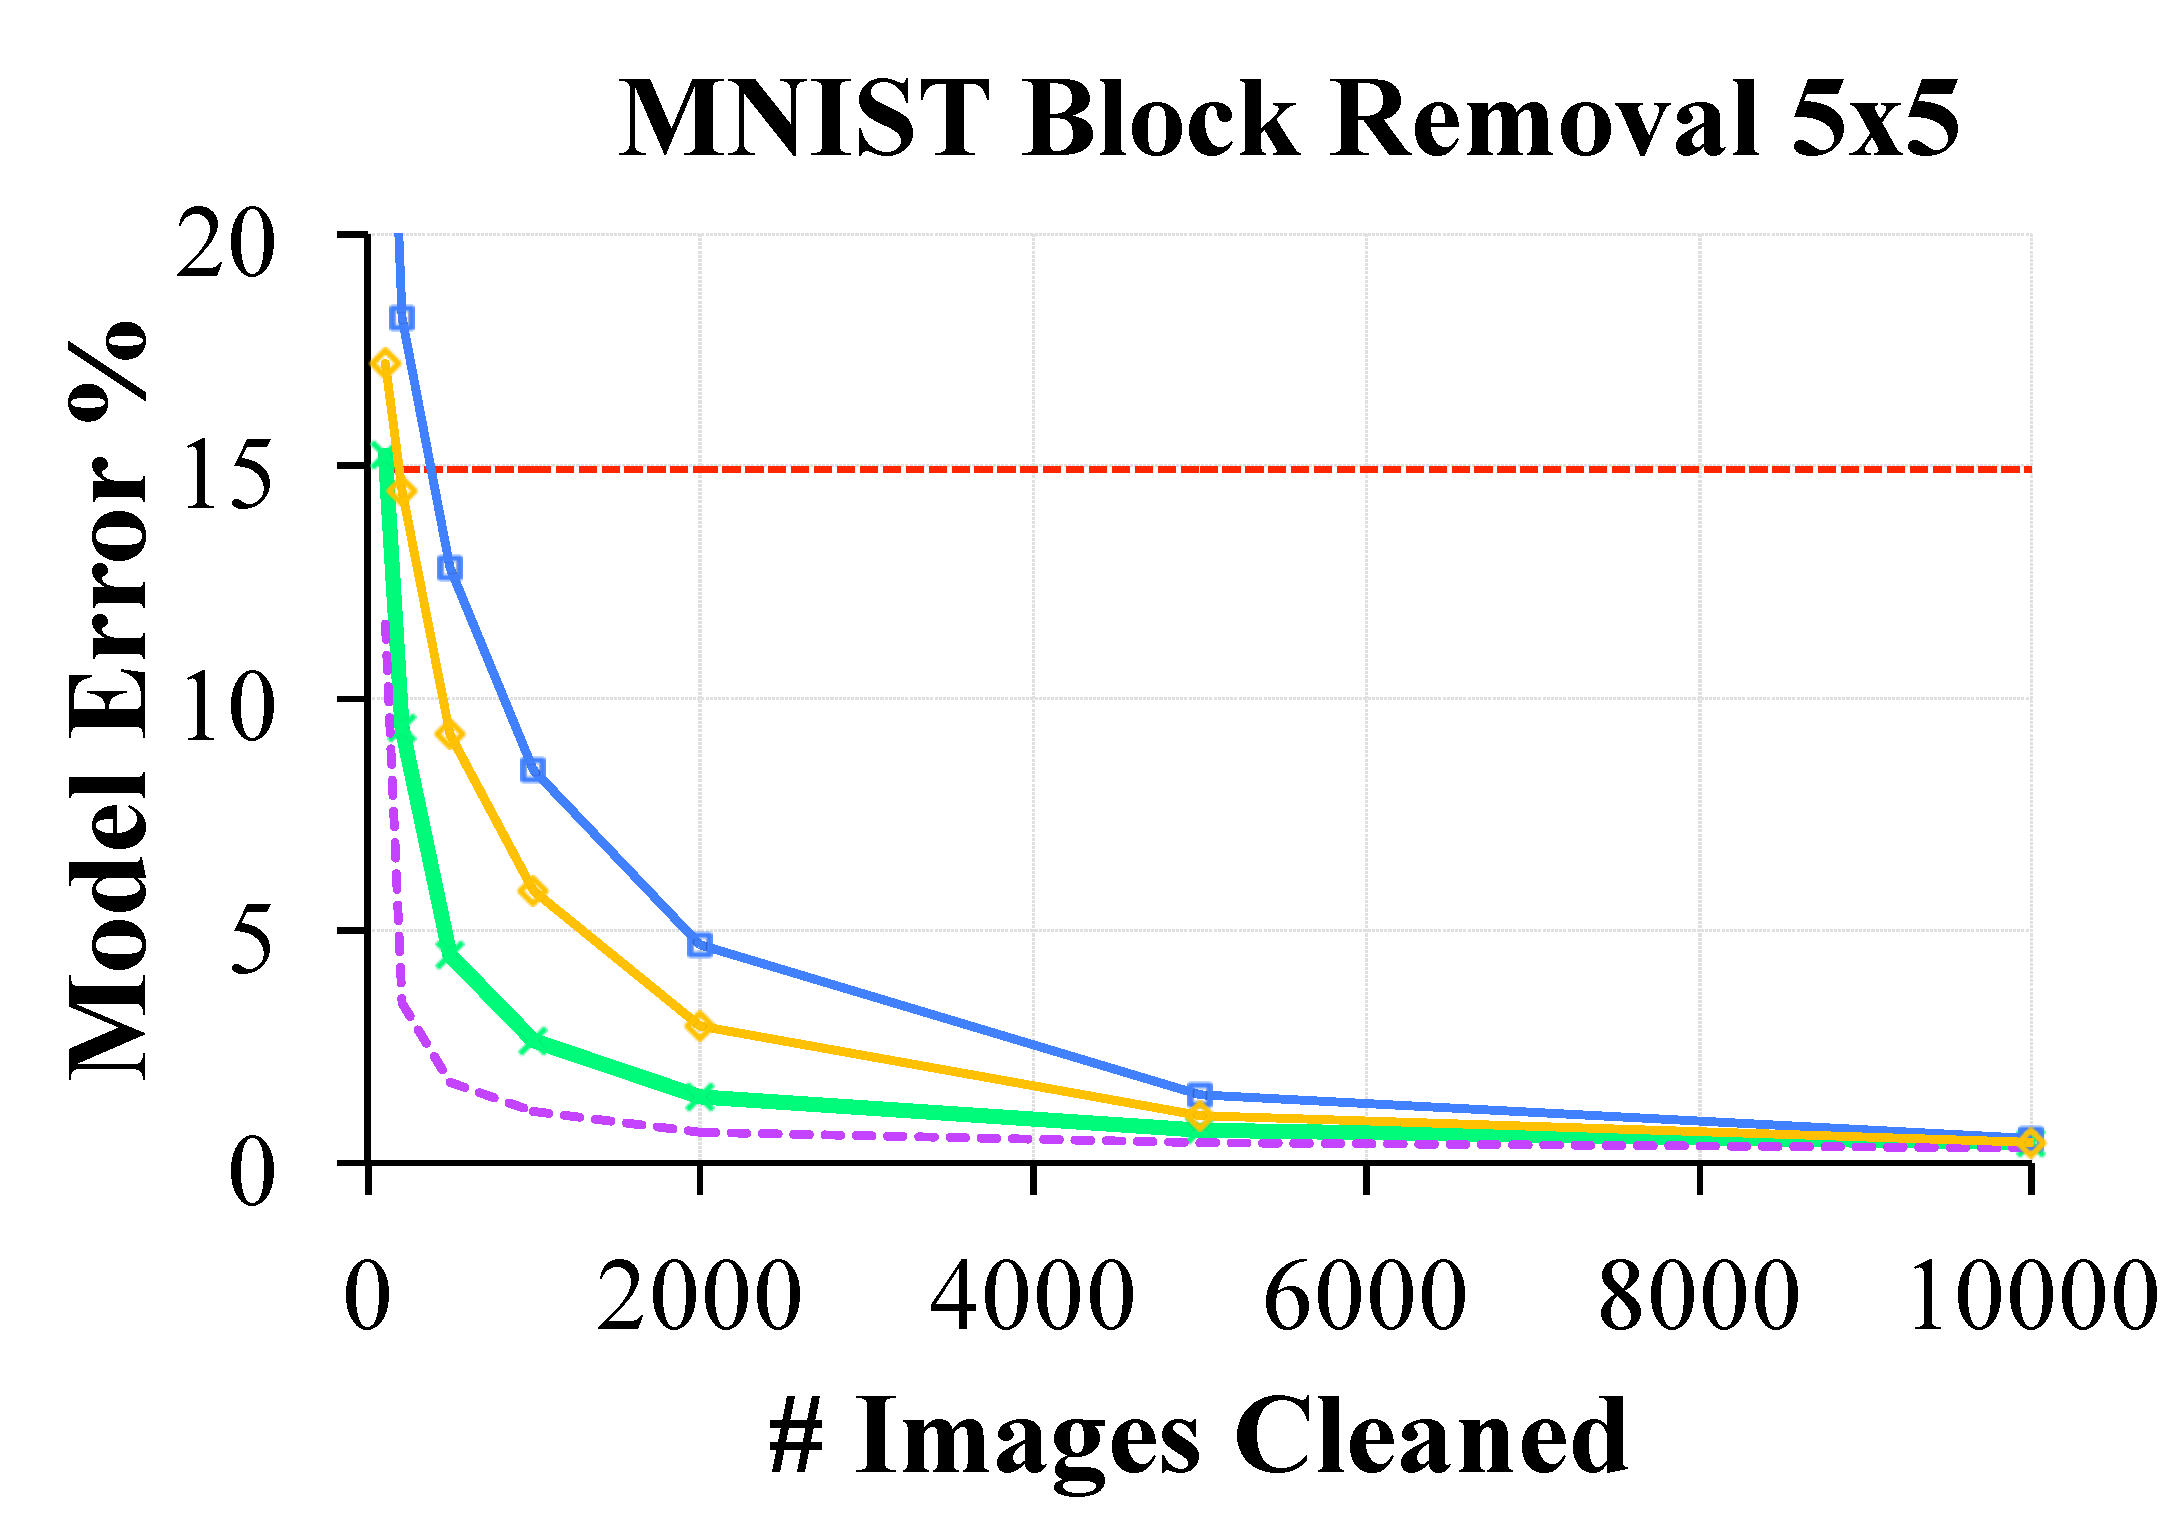
\includegraphics[width=0.49\columnwidth]{exp/exp7a.pdf}
 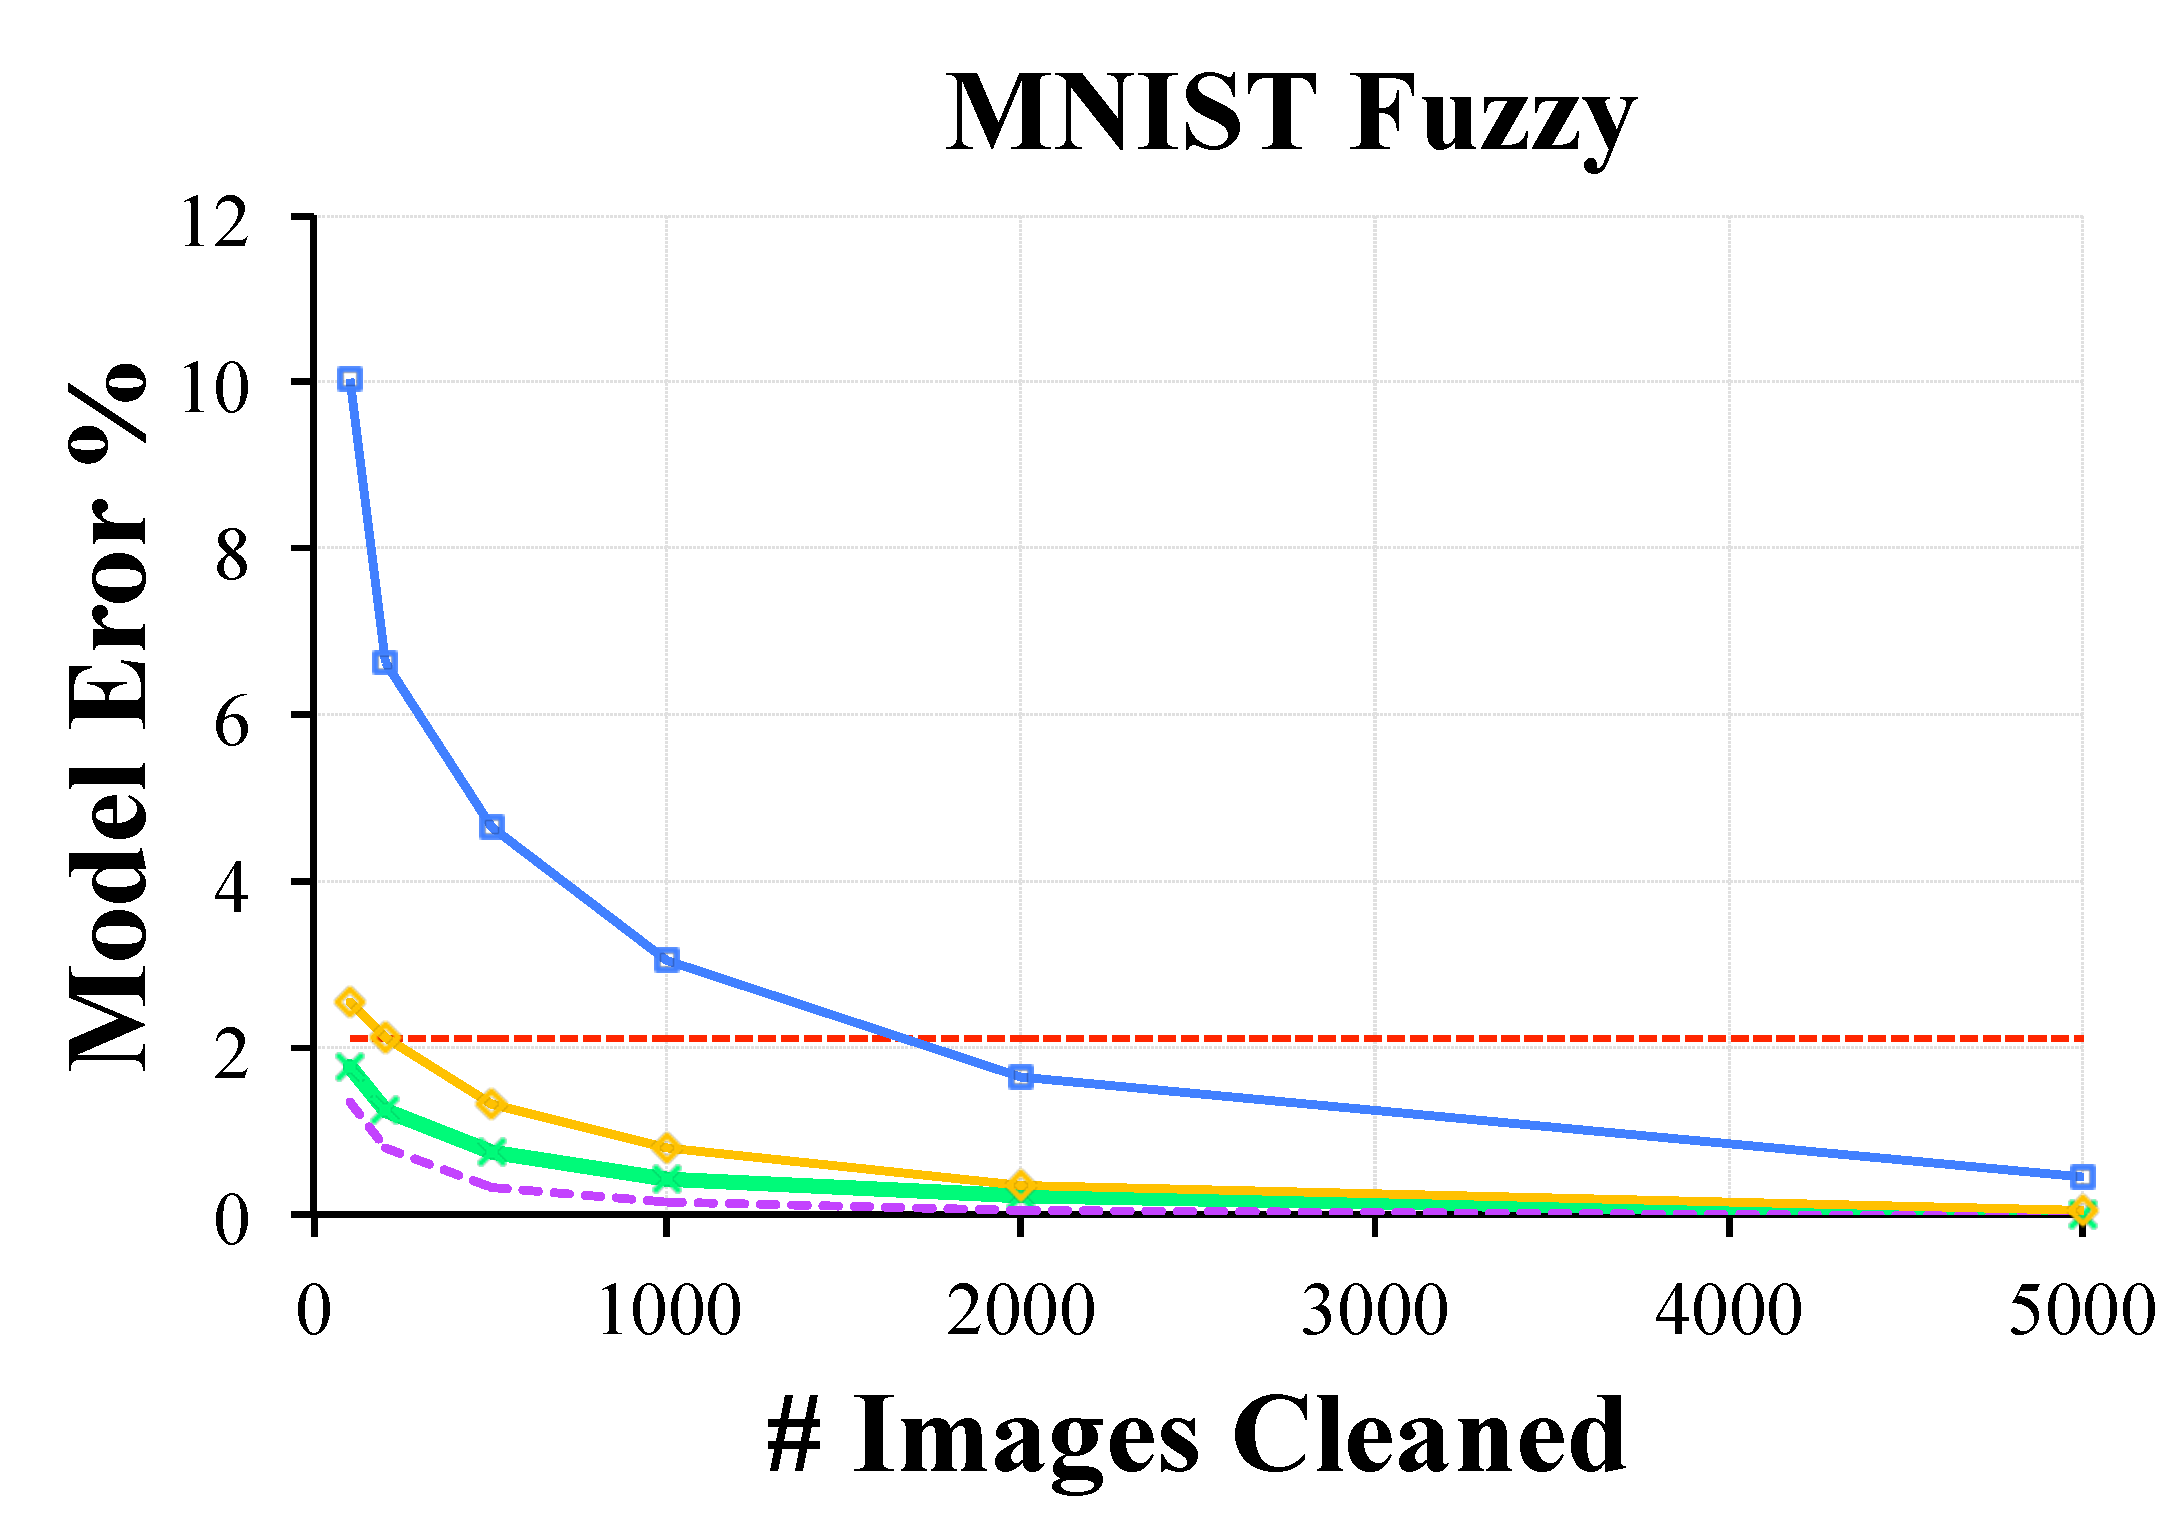
\includegraphics[width=0.49\columnwidth]{exp/exp7b.pdf}
 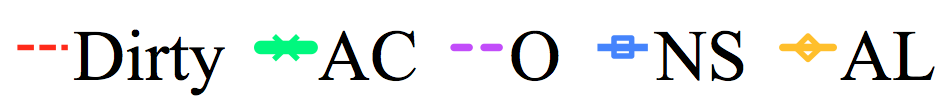
\includegraphics[width=0.49\columnwidth]{exp/legend-general.png}\vspace{-0.5em}
 \caption{In an image processing pipeline on the MNIST dataset with simulated errors, \sys outperforms Active Learning and Naive-Sample.  \label{mnist}}\vspace{-1em}
\end{figure}

\subsection{Simulated Machine Learning Pipeline}
This experiment is representative of modern machine learning pipelines such as Keystone~\cite{keystone} and Google's Tensor Flow~\cite{tensor}. 
The task is to classify 60,000 images of handwritten digits from the MNIST dataset into 10 categories with an one-to-all multiclass SVM classifier~\footnote{\scriptsize\url{http://ufldl.stanford.edu/wiki/index.php/Using_the_MNIST_Dataset}}. 
In contrast to the prior scenarios, which directly extracted feature vectors from the raw dataset, image feature extraction involves a pipeline of transformation steps including edge detection, projection, and raw image patch extraction~\cite{keystone,tensor}.
The cleaning function $C(\dot)$ involves replacing a potentially corrupted image with a non-corrupted version.
We find that pipelines tend to propagate small amounts of corruption, and in fact, and even randomly generated errors can morph into systematic biases.
% What is unique about image processing is that data are often processed through a pipeline of operators edge detectors, projections, and raw image patches~\cite{keystone,tensor}.
% This experiment explores data cleaning in this context, where dirtiness is in the raw data but get propagated through the pipeline.

% We use the MNIST handwritten digit recognition dataset with a MATLAB image processing pipeline.
% In this scenario, the analyst must inspect a potentially corrupted image and replace it with a higher quality one.
% The MNIST dataset consists of 64x64 grayscale images.
There are two types of simulated corruptions that mimic standard corruptions in image processing (occlusion and low-resolution): \texttt{5x5 Removal} deletes a random 5x5 pixel block by setting the pixel values to 0, and \texttt{Fuzzy} blurs the entire image using a 4x4 moving average patch. 
We apply these corruptions to a random 5\% of the images.
\sys's adaptive detector uses a 10 class classifier (one for each digit) to detect the corruption.

Figure \ref{mnist} shows that \sys makes more progress towards the clean model with a smaller number of examples cleaned.
To achieve a 2\% error for 5x5 Removal, \sys can inspect 2200 fewer images than Active Learning and 2750 fewer images than Naive-Sampling.
For the fuzzy images, both Active Learning and \sys reach 2\% error after examining $<100$ images, while Naive-Sampling requires 1750.
Even though these corruptions are applied independent of the data, the \texttt{5x5 Removal} propagates through the pipeline as a systematic error.
The image features are constructed with edge detectors, which are highly sensitive to this type of corruption.
Some digits naturally have fewer edges than others are disproportionately affected since the removal process adds spurious edges.
On the other hand, the \texttt{Fuzzy} corruption propagates through the pipeline more similar to random error.
This experiment highlights that featurization and other data processing pipelines between the raw data and model can introduce systematic biases in the presence of data corruption.

\subsection{Simulated Error Scenarios}
In the next set of experiments, we use standard Machine Learning benchmark datasets and corrupt them with varying levels of systematic noise.
We use this to evaluate \sys while isolating certain variables.
The two datasets that we used were:

\vspace{0.25em}

\noindent\textbf{Income Classification (Adult): } In this dataset of 45,552 records, the task is to predict the income bracket (binary) from 12 numerical and categorical covariates with an SVM classifier. 

\vspace{0.25em}

\noindent\textbf{Seizure Classification (EEG): } In this dataset, the task is to predict the onset of a seizure (binary) from 15 numerical covariates with a thresholded Linear Regression. There are 14980 data points in this dataset. This classification task is inherently hard with an accuracy on the completely clean data is only 65\%.

\subsubsection{Source of Improvements}\label{comp}
This experiment compares the performance of \sys with and without various optimizations for 500 records examined. 
\sys without detection is denoted as (AC-D) (that is at each iteration we sample from the entire dirty data), and \sys without detection and our prioritized sampling is denoted as (AC-D-I).
Figure \ref{opts} plots the relative error of the alternatives and \sys with and without the optimizations.
Without detection (AC-D), \sys is still more accurate than Active Learning.
Removing the sampling, \sys is slightly worse than Active Learning on the Adult dataset but is comparable on the EEG dataset.
The advantage of \sys is that it is a composable framework supporting different instantiations of the detection and prioritization modules while still preserving convergence guarantees.
With these optimizations, \sys is consistently more efficient than Active Learning.

\begin{figure}[t]\vspace{0.5em}
\centering
 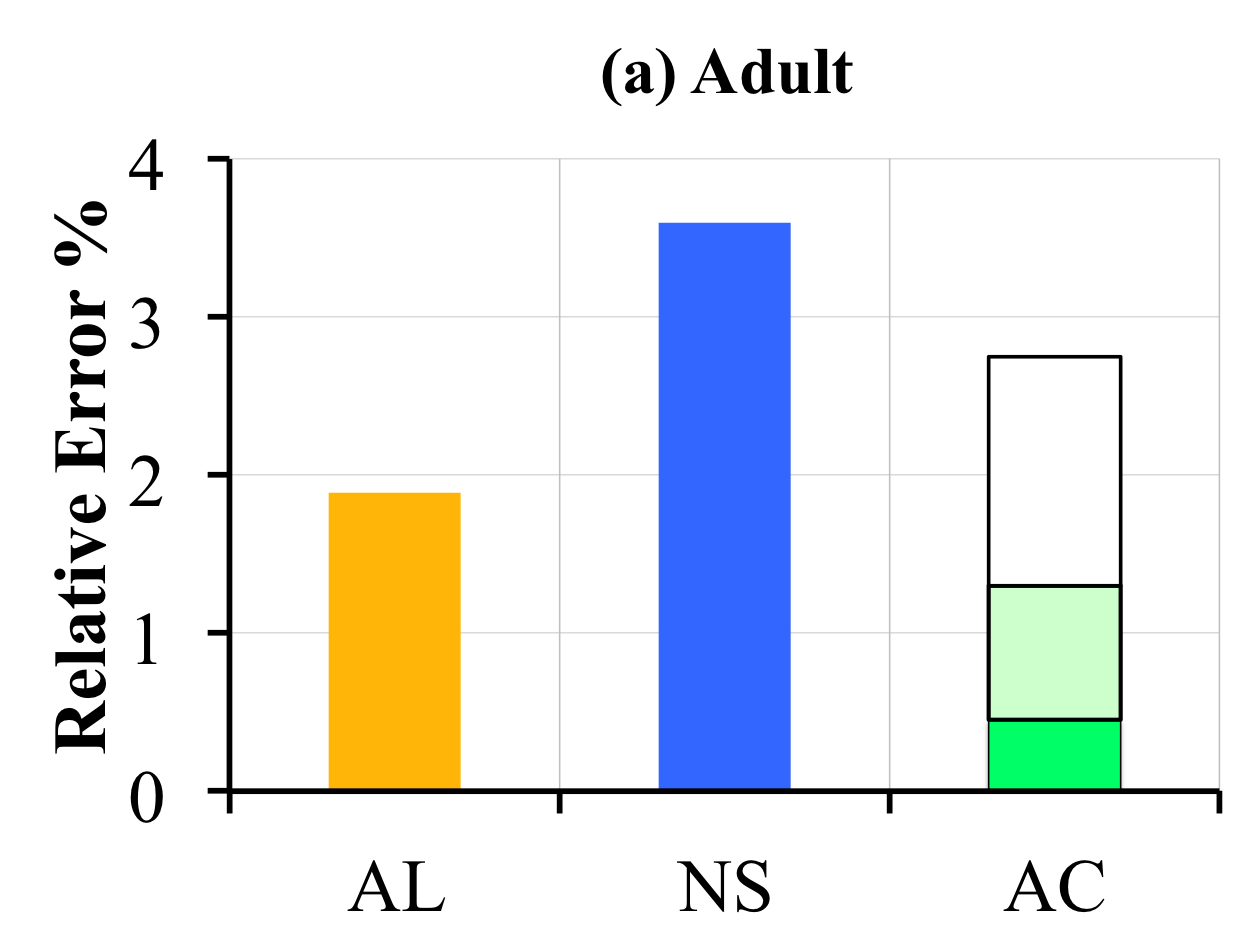
\includegraphics[width=0.49\columnwidth]{exp/exp8a.png}
 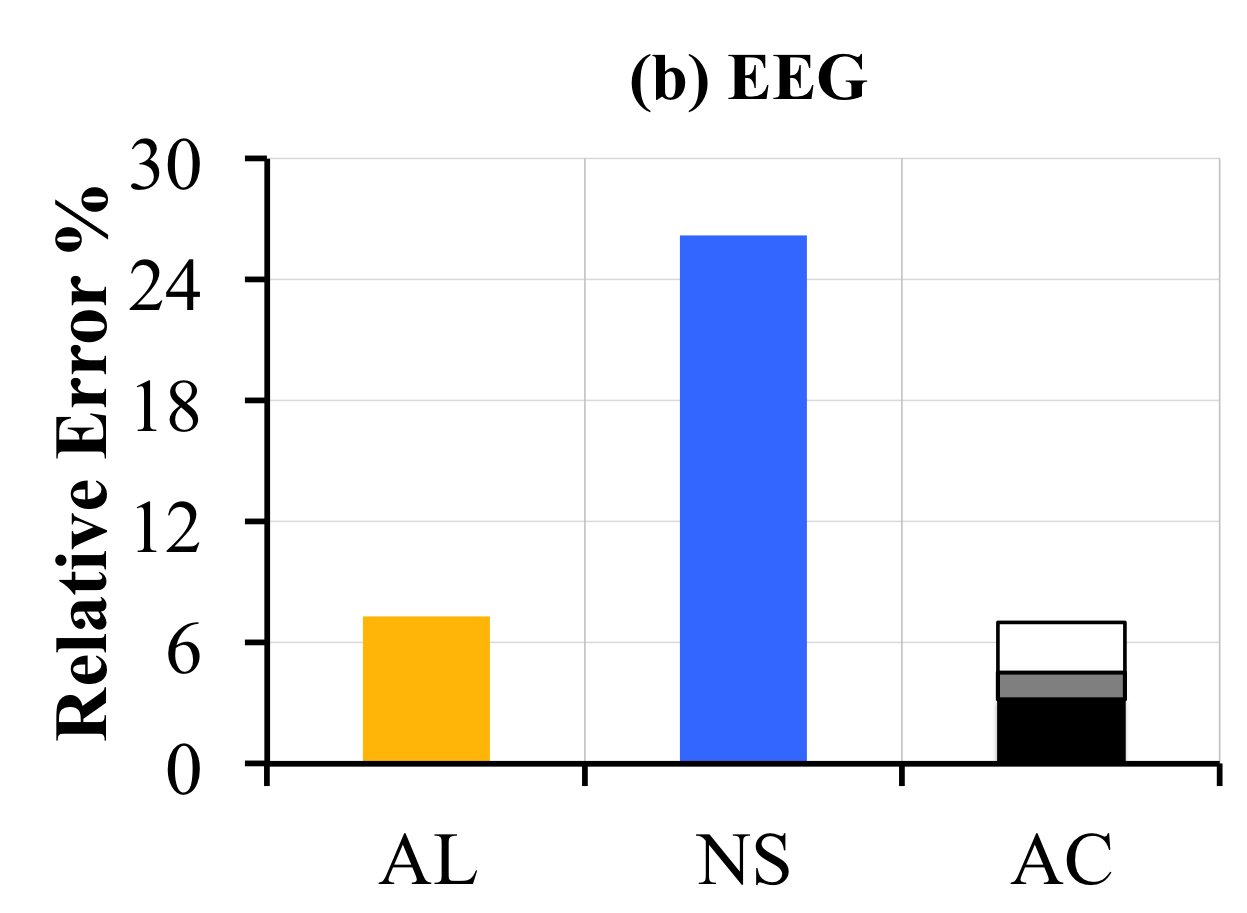
\includegraphics[width=0.49\columnwidth]{exp/exp8b.png}
 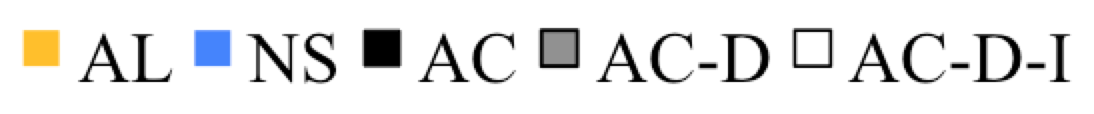
\includegraphics[width=0.5\columnwidth]{exp/legend-8.png}\vspace{-1em}
 \caption{ -D denotes no detection, and -D-I denotes no detection and no importance sampling. Both optimizations significantly help \sys outperform Naive-Sampling and Active Learning. \label{opts}}\vspace{-1.5em}
\end{figure}

\subsubsection{Mixing Dirty and Clean Data}\label{exp:rtr}
Naive-Mix is an unreliable methodology lacking the same guarantees as Active Learning or Naive-Sampling even in the simplest of cases.
We also saw that it is significantly less efficient than \sys, Naive-Sampling, and Active Learning on the real datasets.
For thoroughness, these experiments include the model error as a function of records examined in comparison to \sys.
We also evaluate this approach with our detection component.
Naive-Mix+D randomly samples data using the dirty data detector, applies the user-specified cleaning, and writes-back the cleaned data.

Figure \ref{pc-perf} plots the same curves as the previous experiment comparing \sys, Active Learning, and two mixed data algorithms.
Intuitively, Naive-Mix makes less progress with each update.
Consider the case where 10\% of the dataset is corrupted and a small sample of data 1\%.
\sys and Naive-Sampling extrapolate from the cleaned sample (\sys extrapolates a gradient) while Naive-Mix considers the entire dirty data which might be much larger.

%\sys converges faster.
%\sys tunes the weighting when averaging dirty and clean data into the gradient.

\begin{figure}[ht!]
\centering\vspace{-0.5em}
 %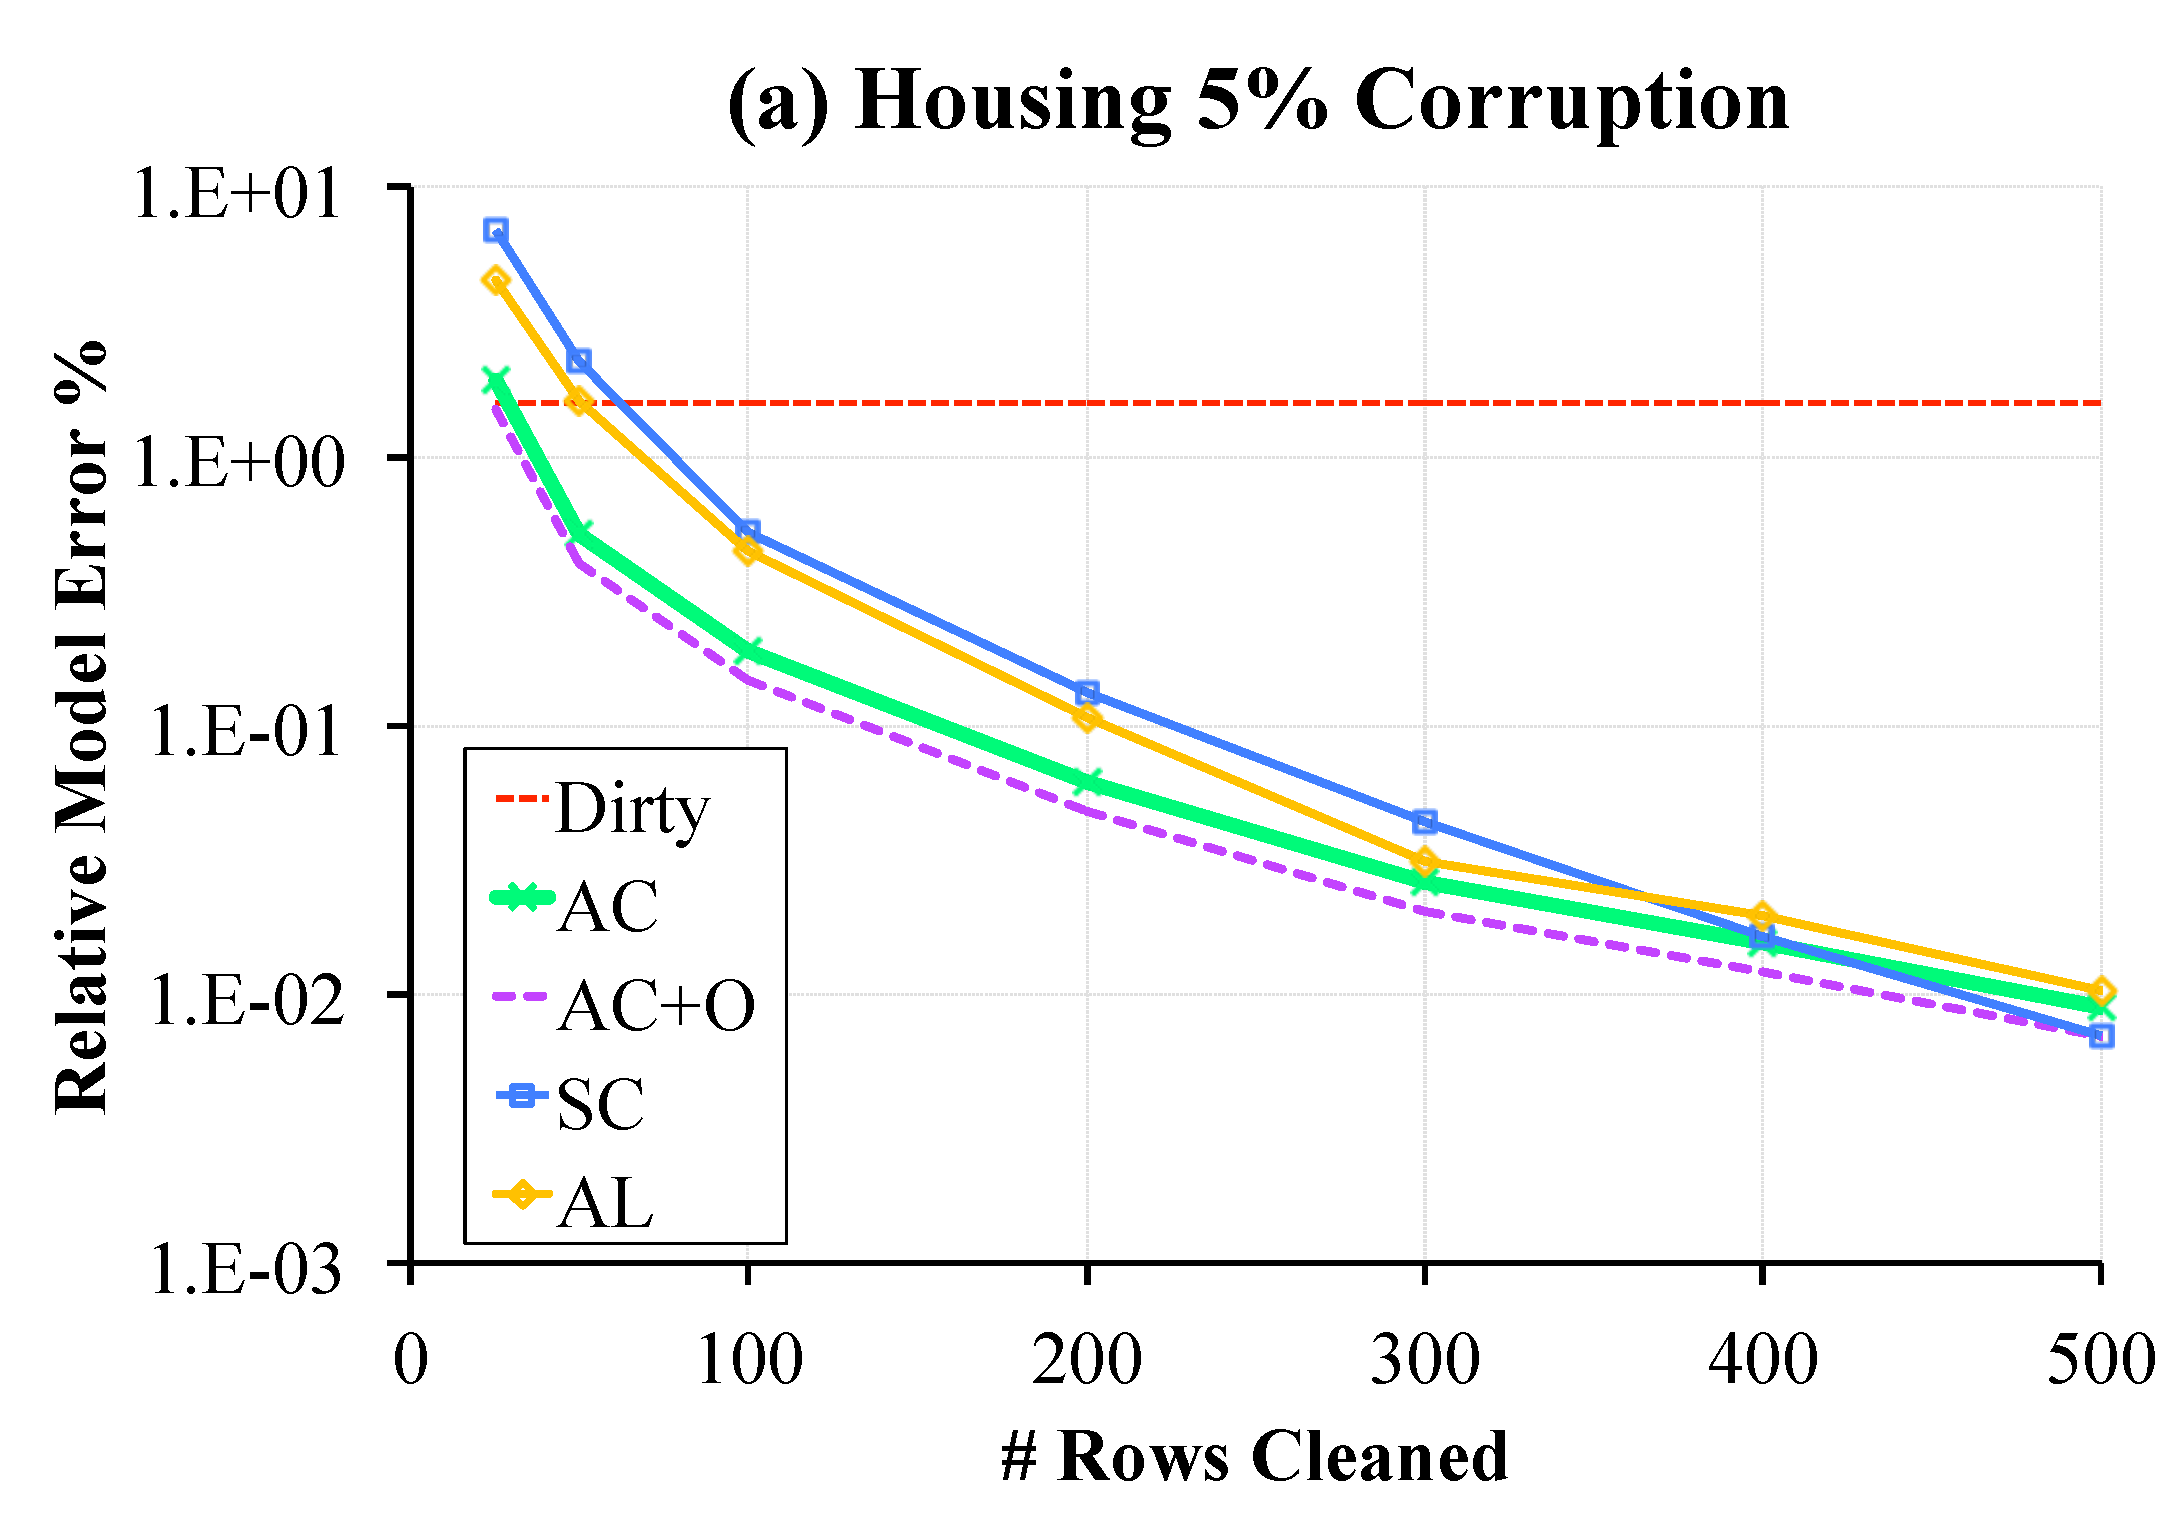
\includegraphics[scale=0.15]{exp/exp3a.pdf}
 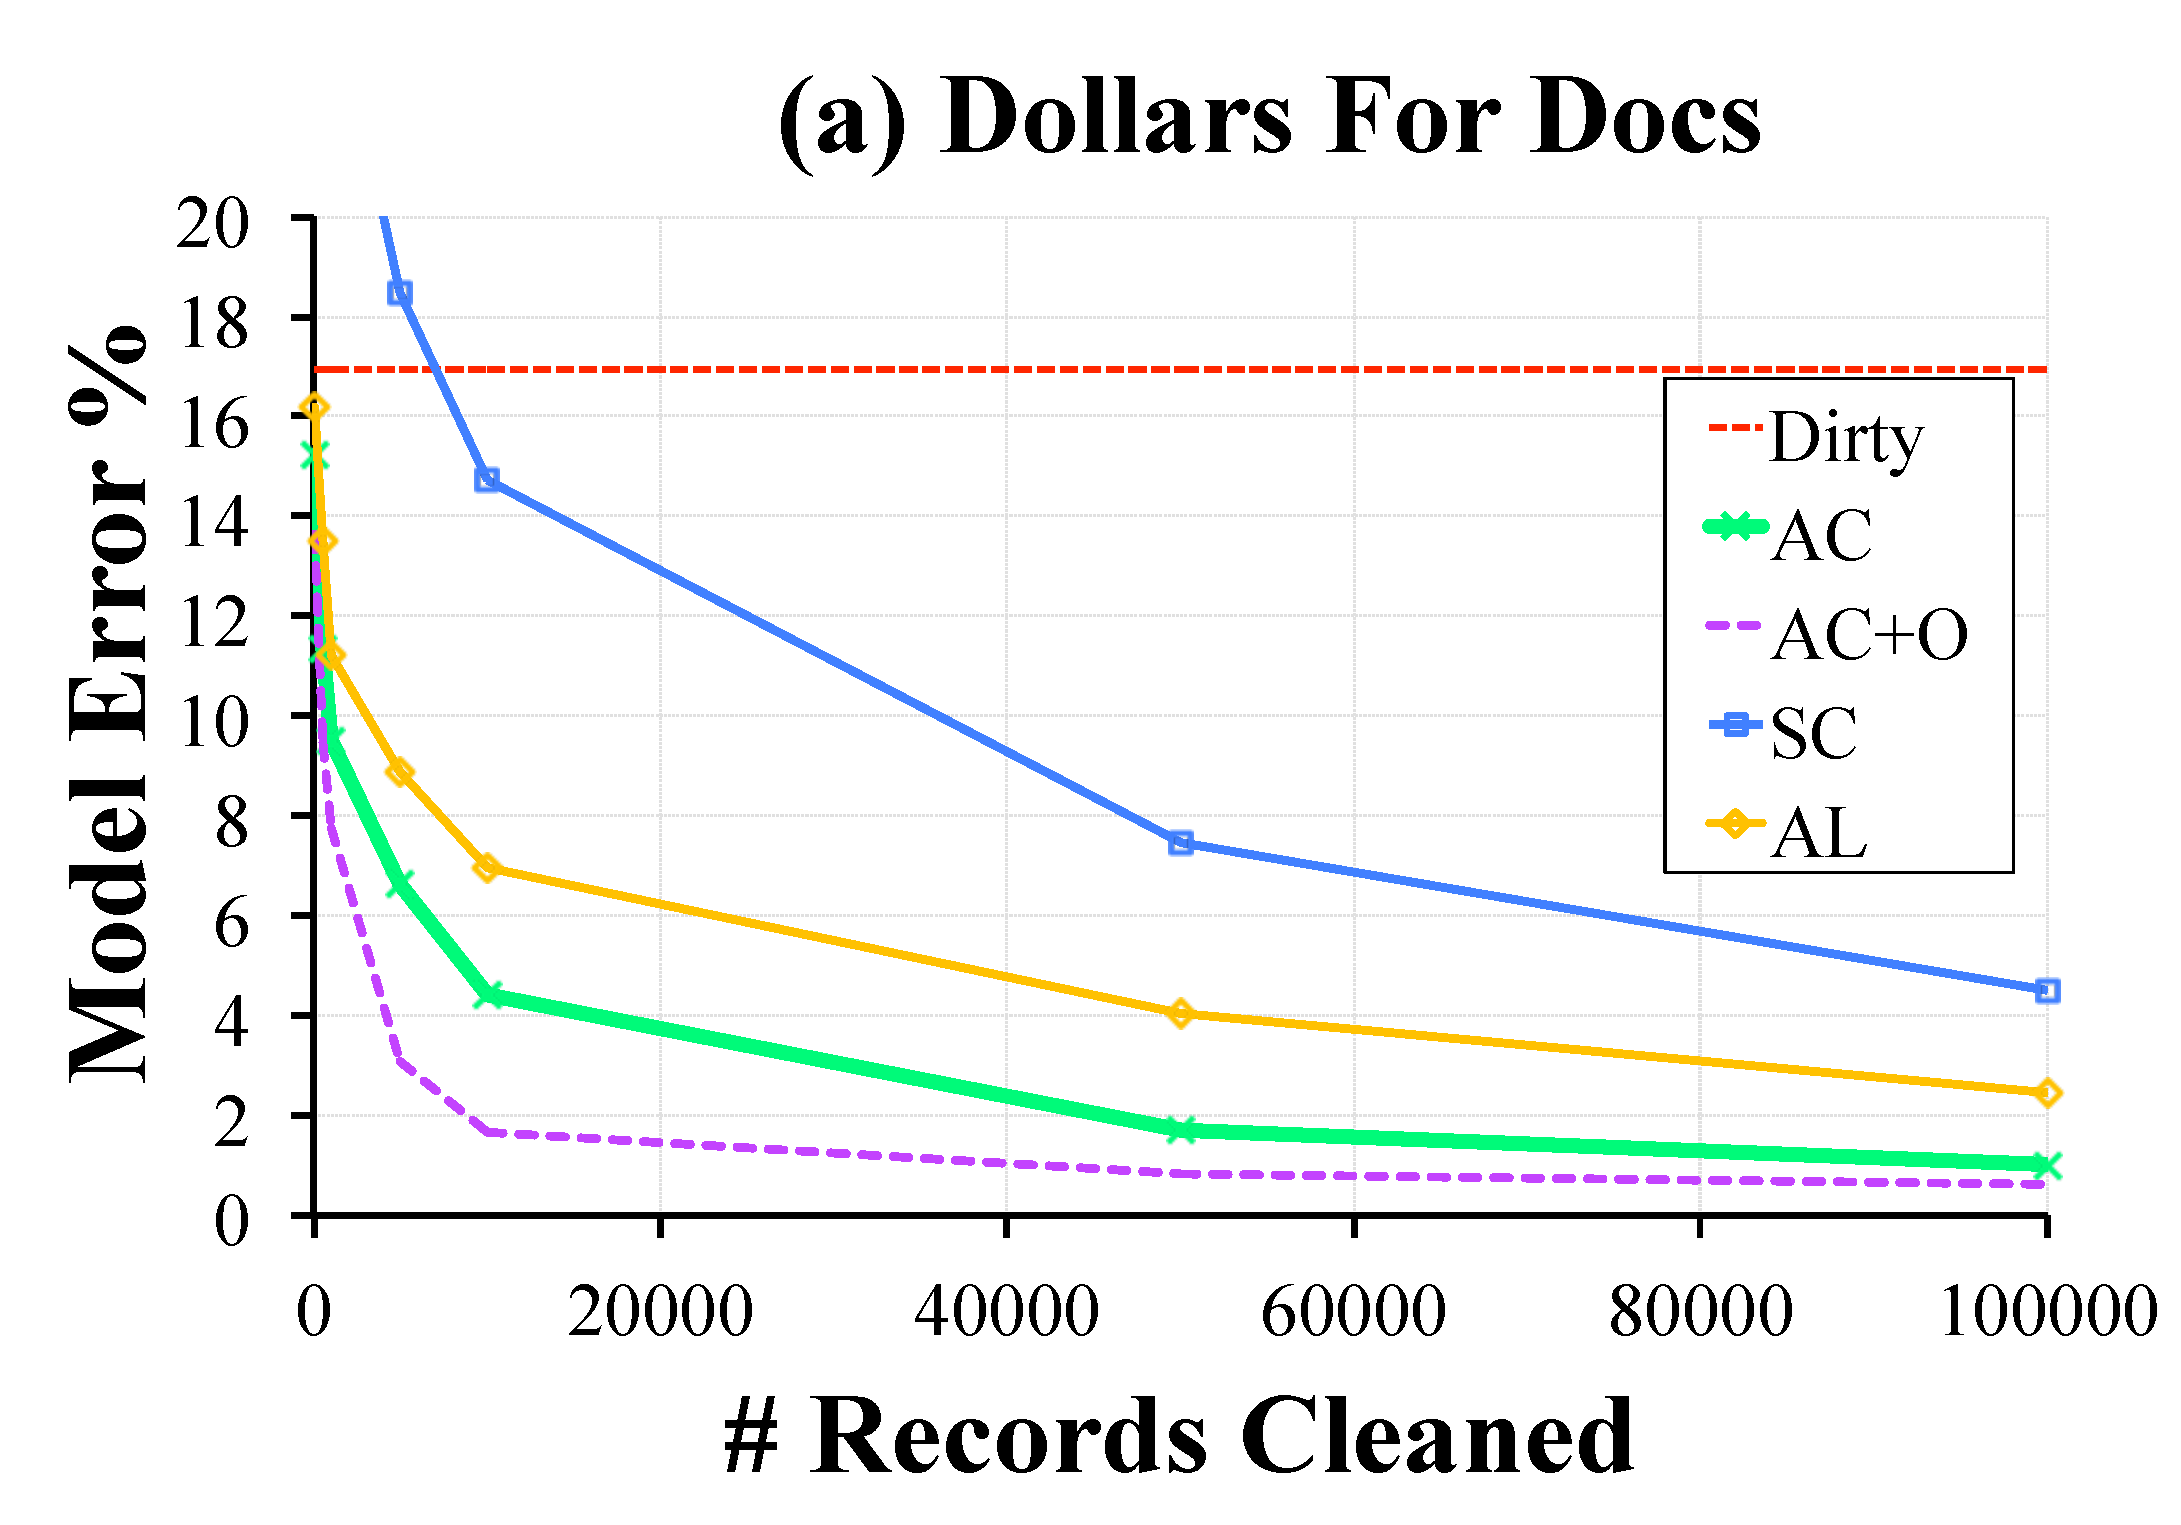
\includegraphics[width=0.49\columnwidth]{exp/exp14a.pdf}
    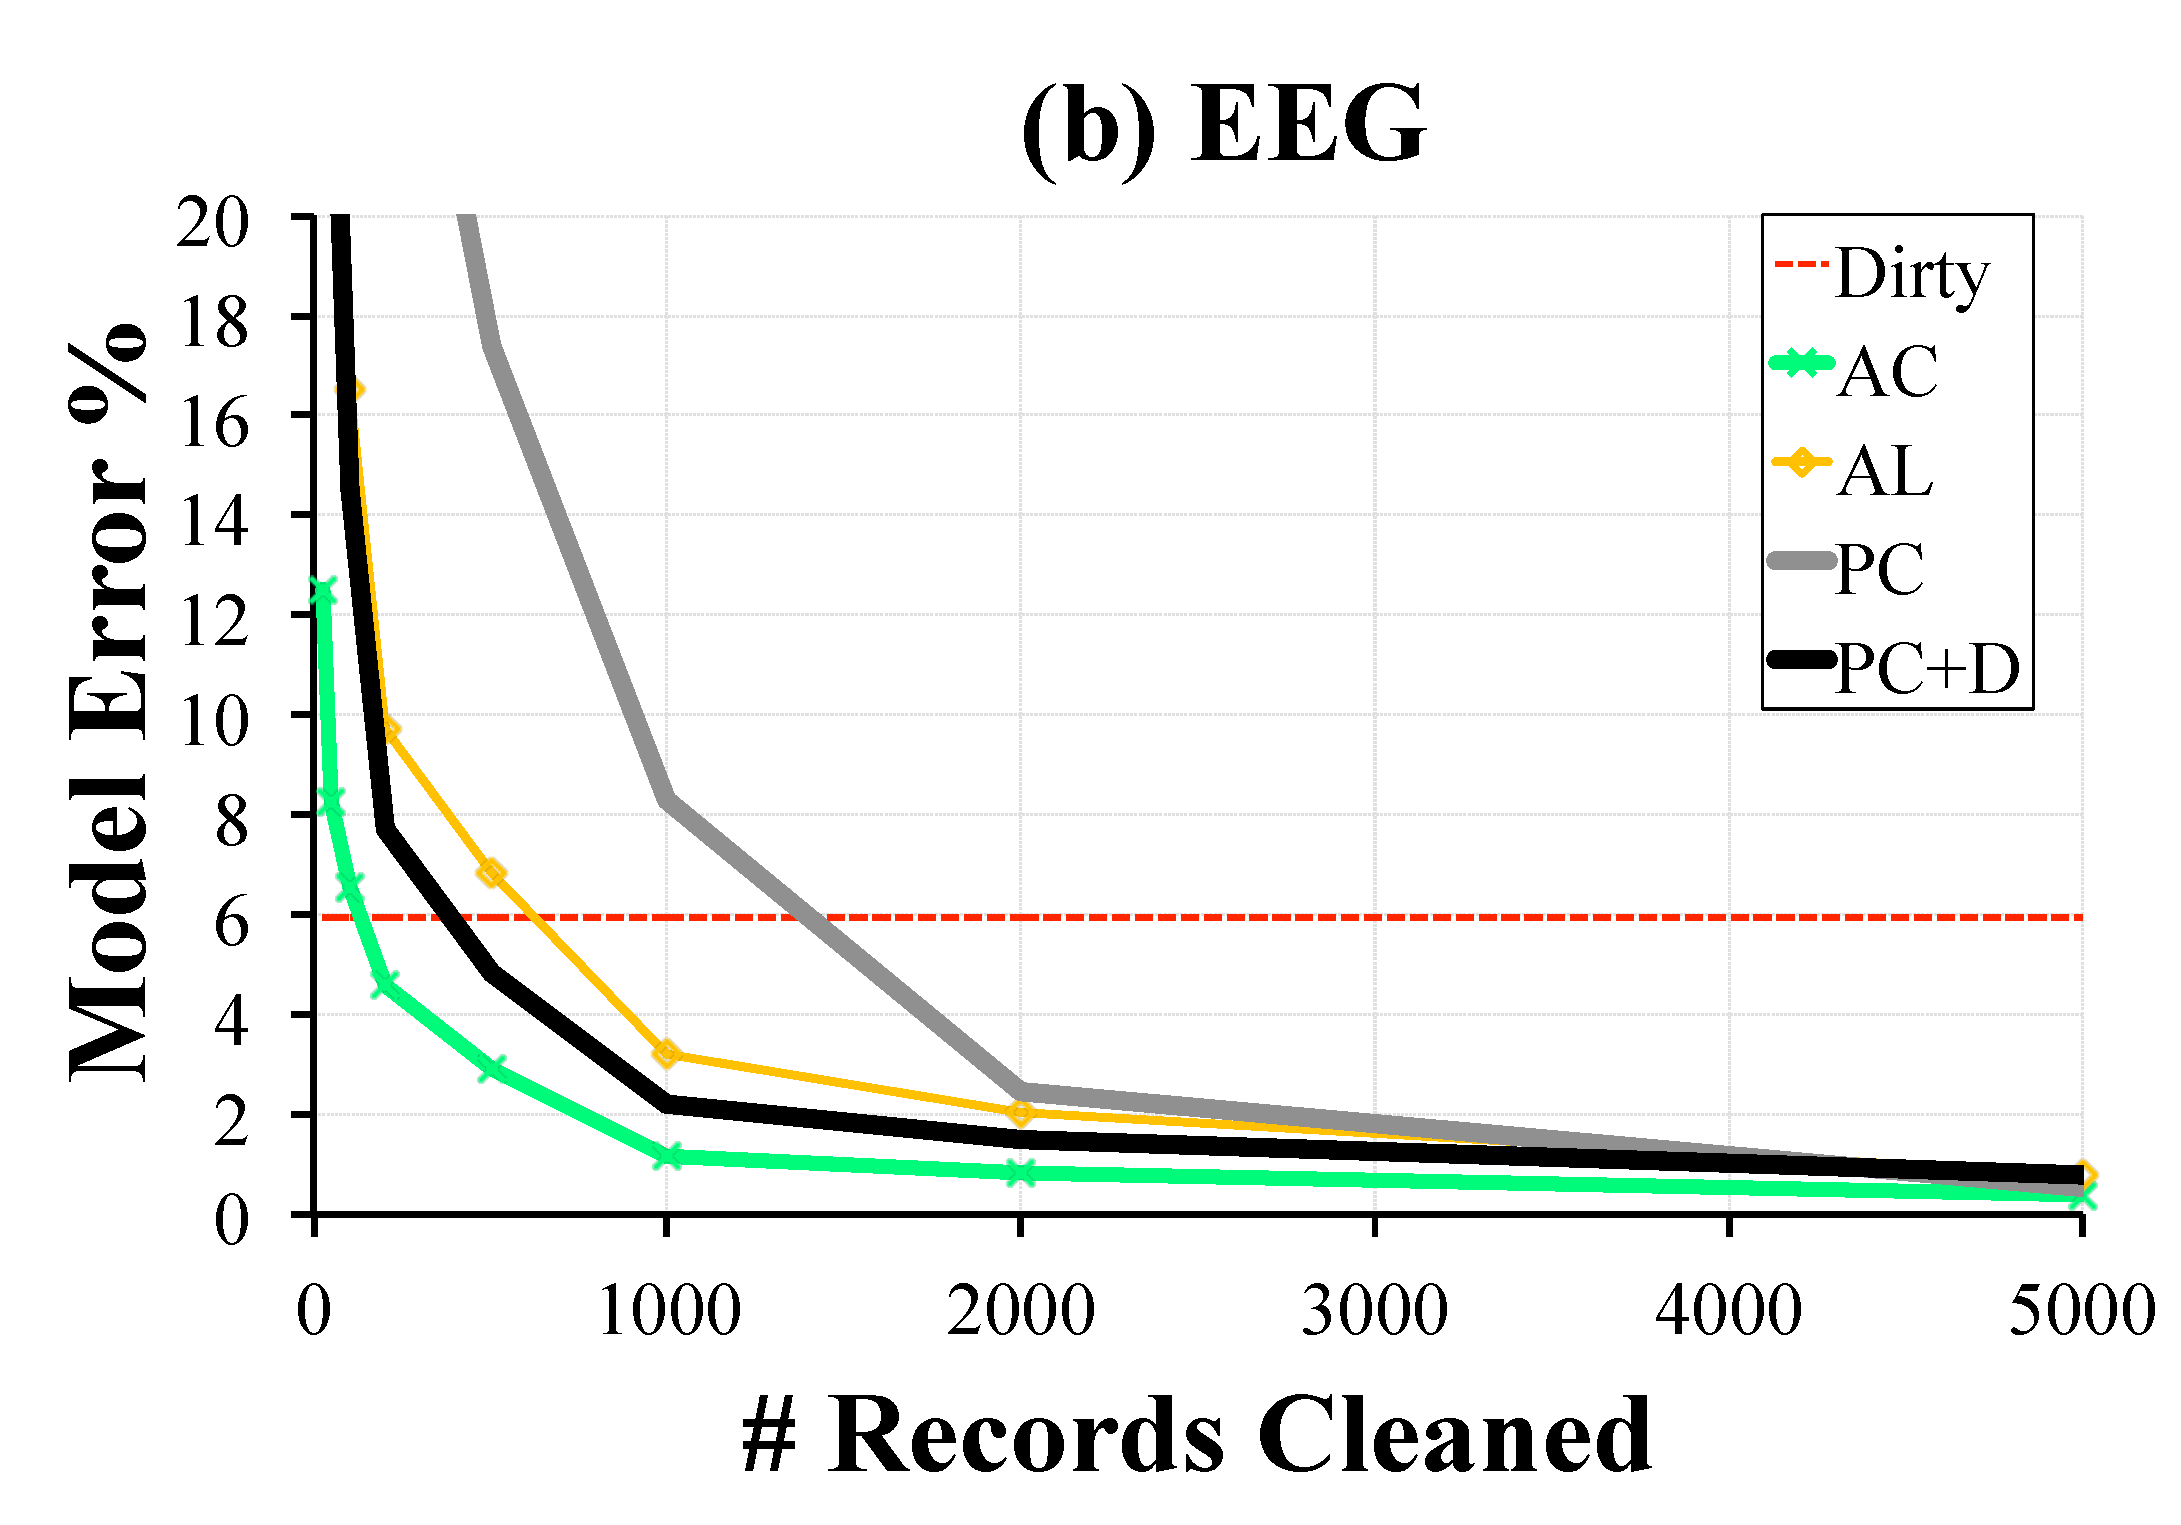
\includegraphics[width=0.49\columnwidth]{exp/exp14b.pdf}
    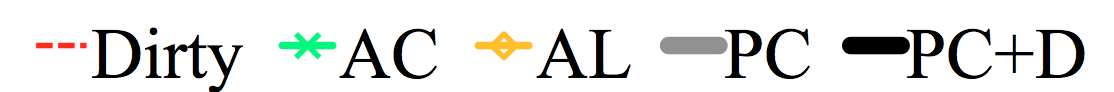
\includegraphics[width=0.49\columnwidth]{exp/legend-14.png}\vspace{-0.5em}
 \caption{The relative model error as a function of the number of examples cleaned. \sys converges with a smaller sample size to the true result in comparison to partial cleaning (NM, NM+D).  \label{pc-perf}}
\end{figure}

\subsubsection{Corruption Rate}
This experiment explores the tradeoff between Naive-Sampling and \sys.
Figure \ref{bias} varies the systematic corruption rate and plots the number of records examined to achieve 1\% relative error for Naive-Sampling and \sys.
Naive-Sampling does not use the dirty data and thus its error is essentially governed by the the sample size and not the magnitude or prevalence of corruption.
Naive-Sampling outperforms \sys only when corruptions are very severe (45\% in Adult and nearly 60\% in EEG).
When the initialization with the dirty model is inaccurate, \sys does not perform as well. 

\begin{figure}[t]
\centering
 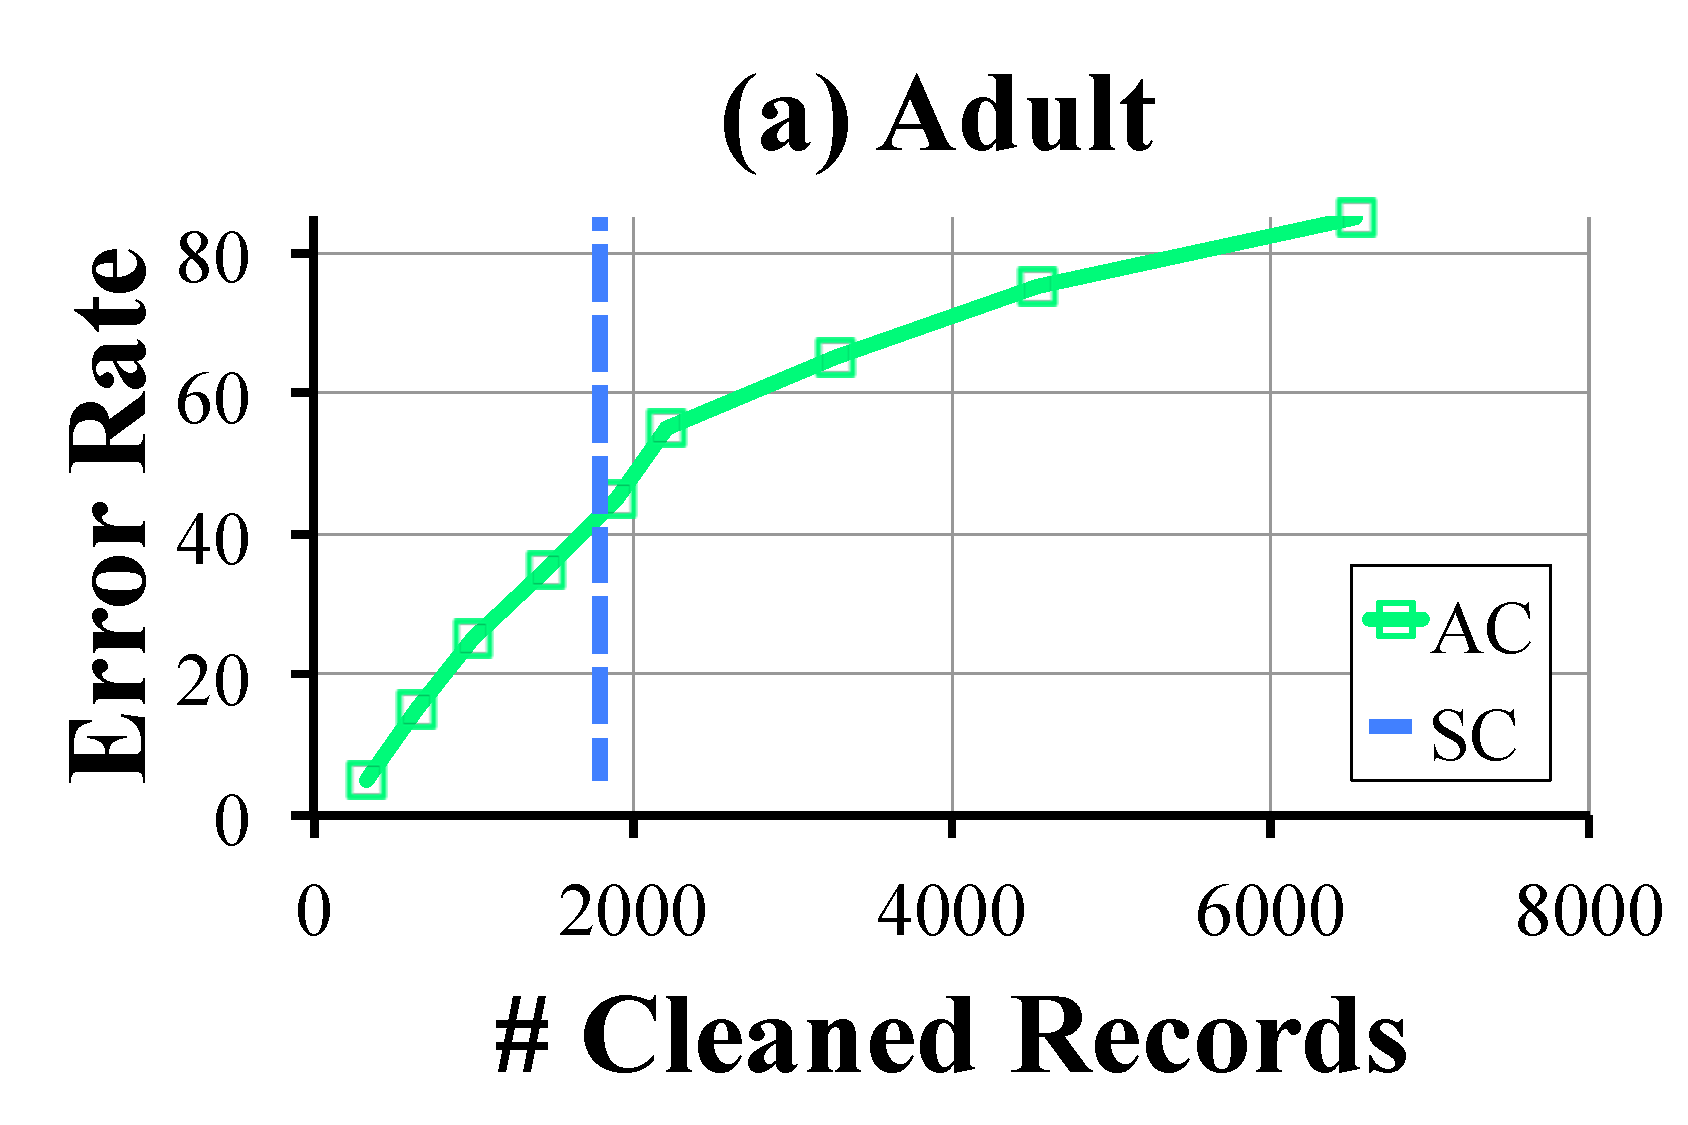
\includegraphics[width=0.49\columnwidth]{exp/exp9a.pdf}
  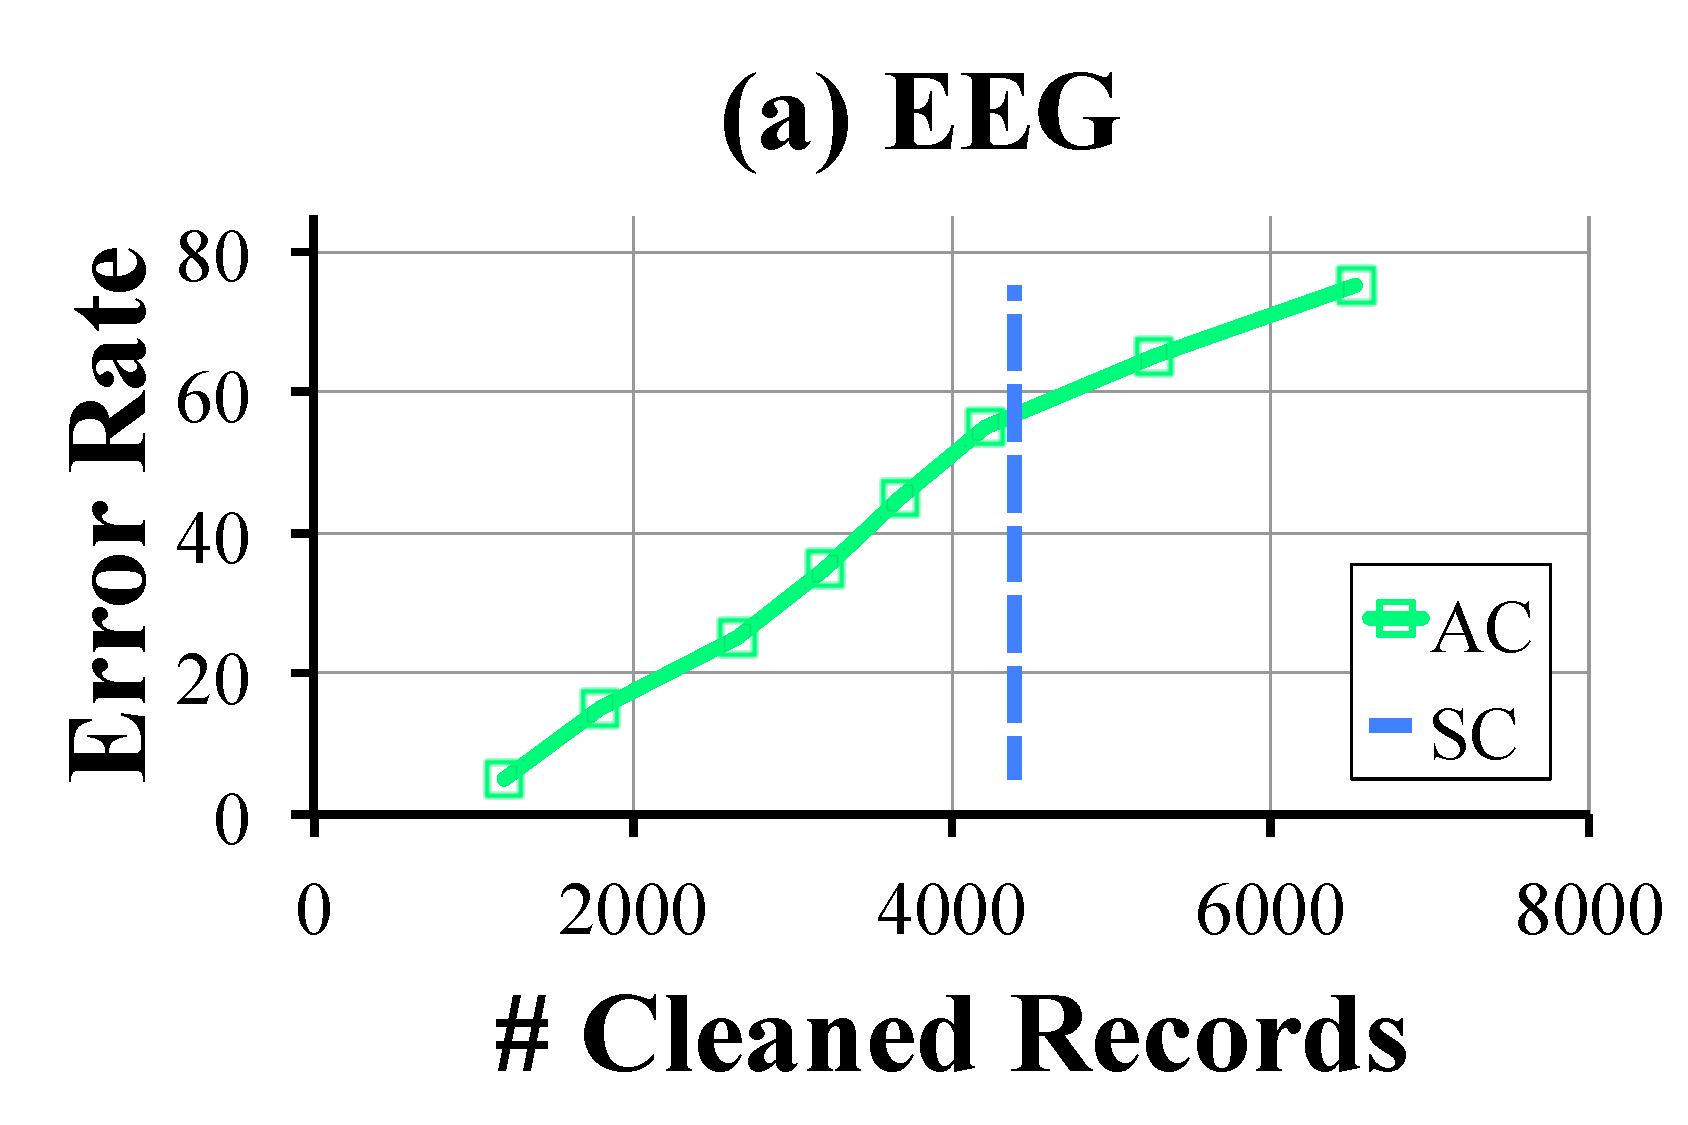
\includegraphics[width=0.49\columnwidth]{exp/exp9b.pdf}\vspace{-1em}
 \caption{\sys outperforms Naive until the corruption is so severe that the dirty model is initialized very far away from the clean model.
  The error of Naive-Sampling does not depend on the corruption rate so it is a vertical line.  \label{bias}}
\end{figure}

\begin{figure}[t]
\centering
 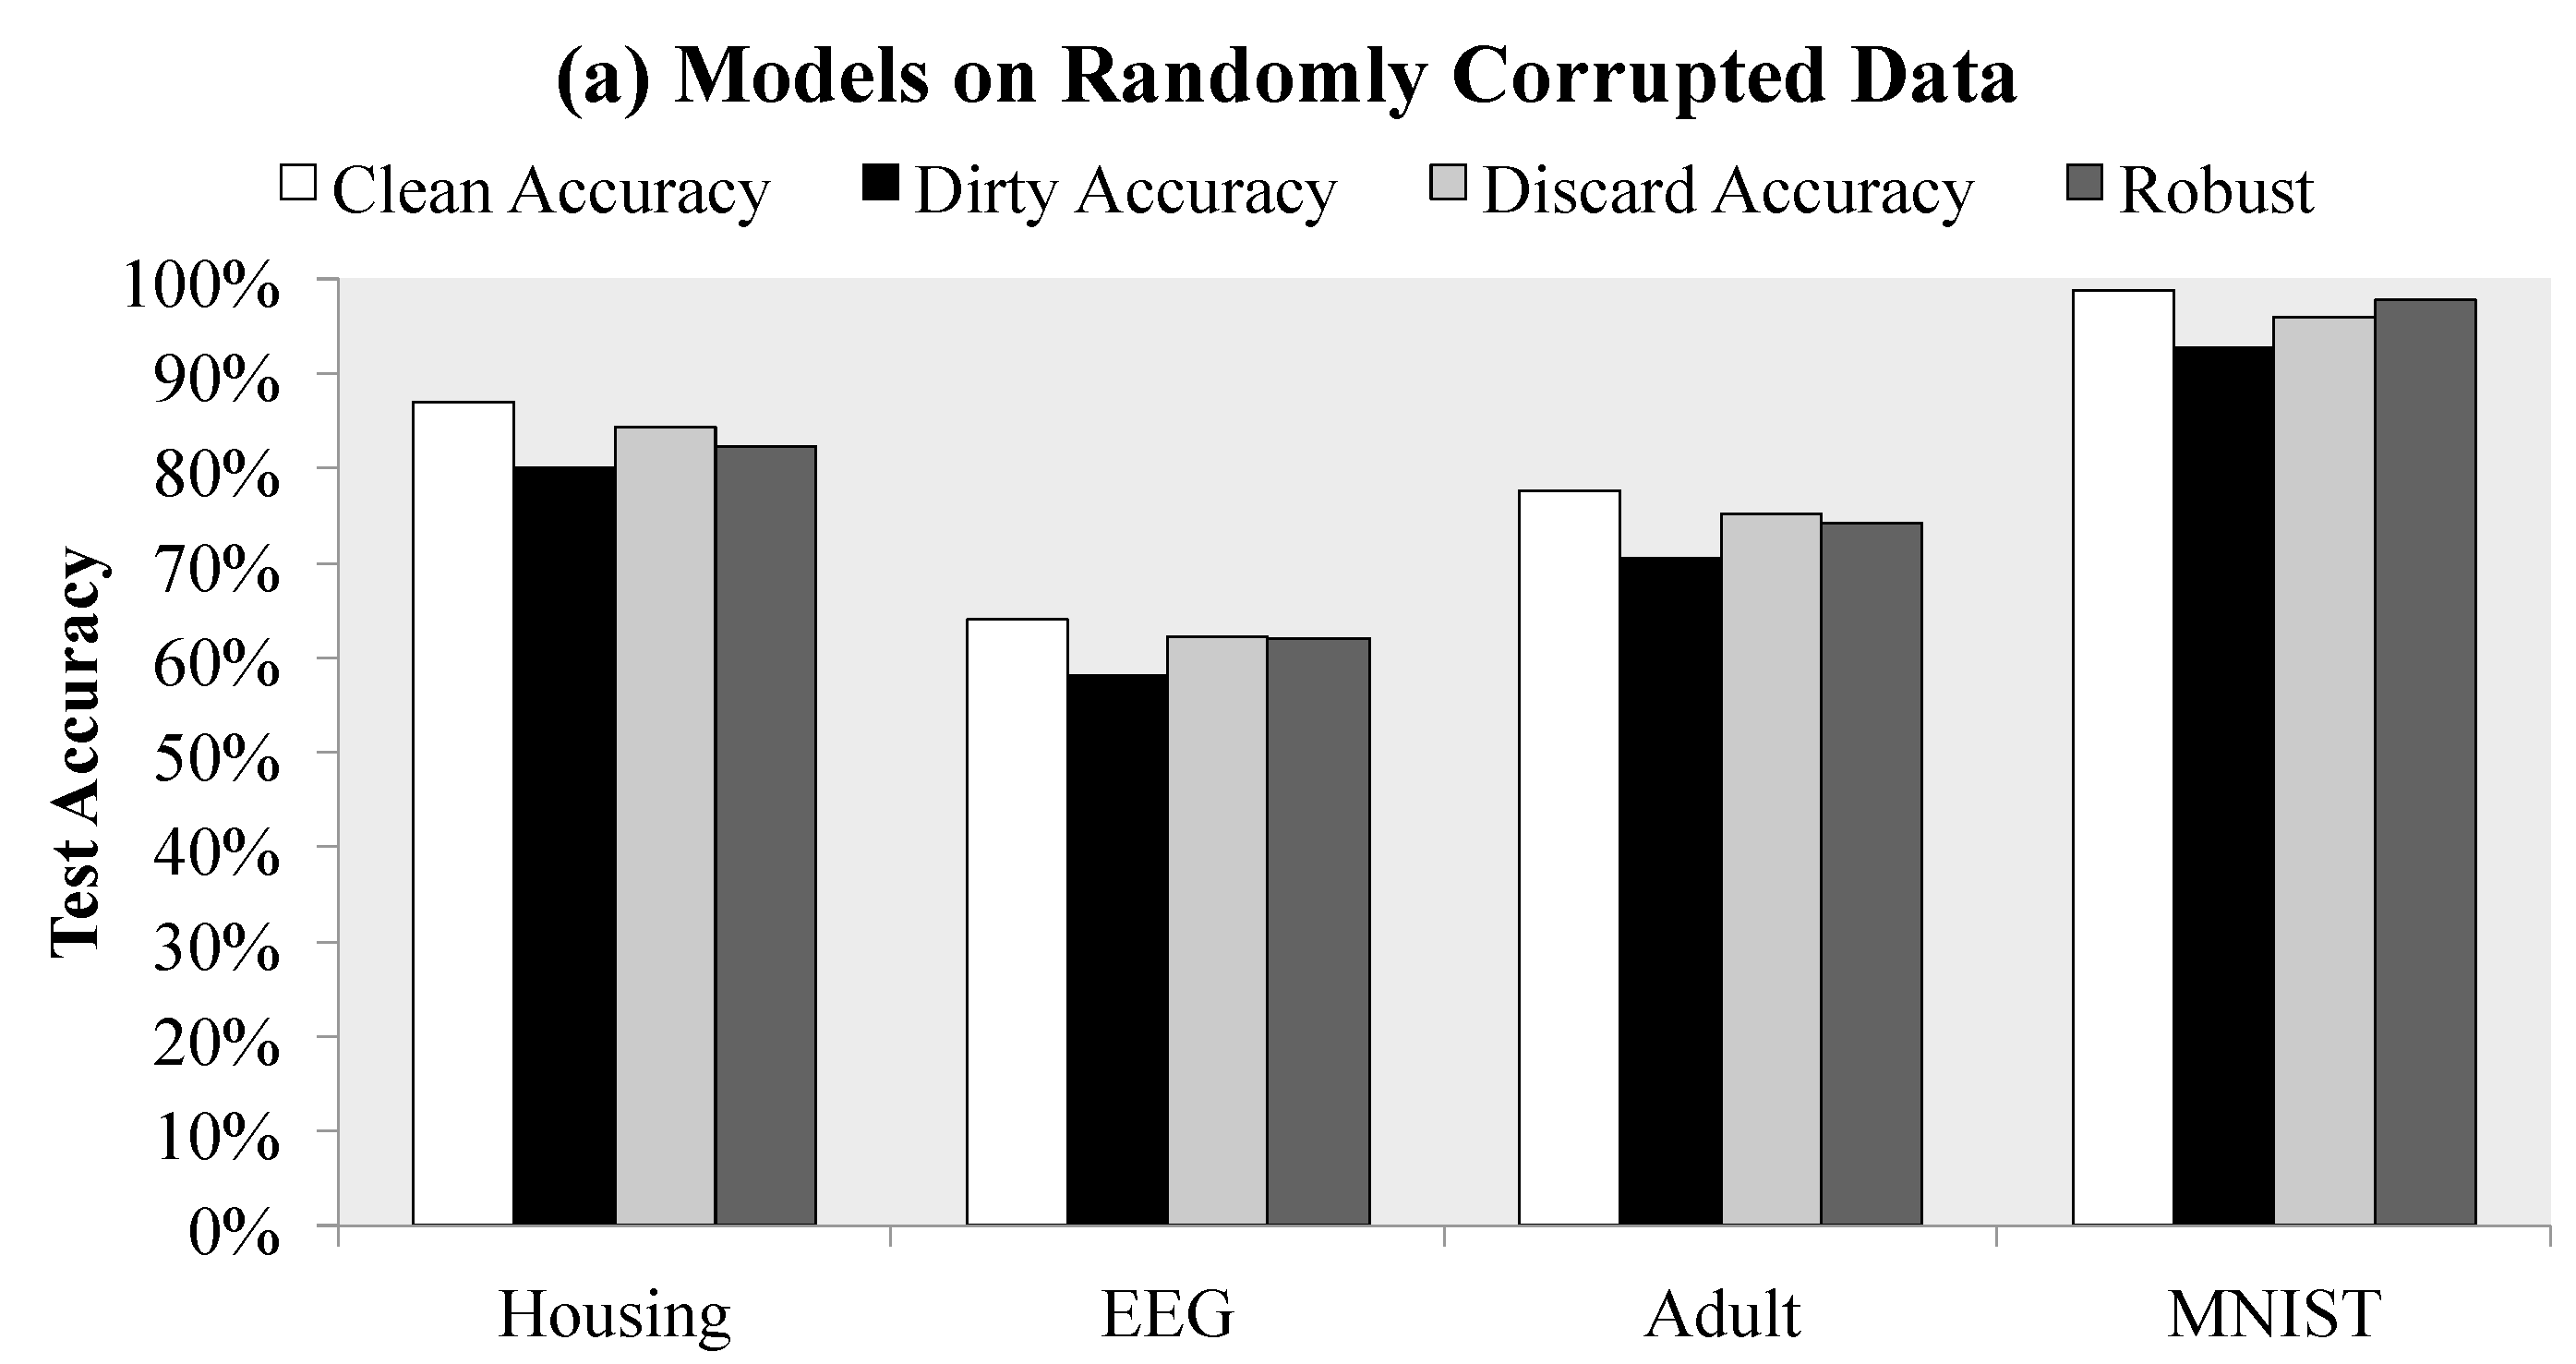
\includegraphics[width=0.49\columnwidth]{exp/exp2.pdf}
 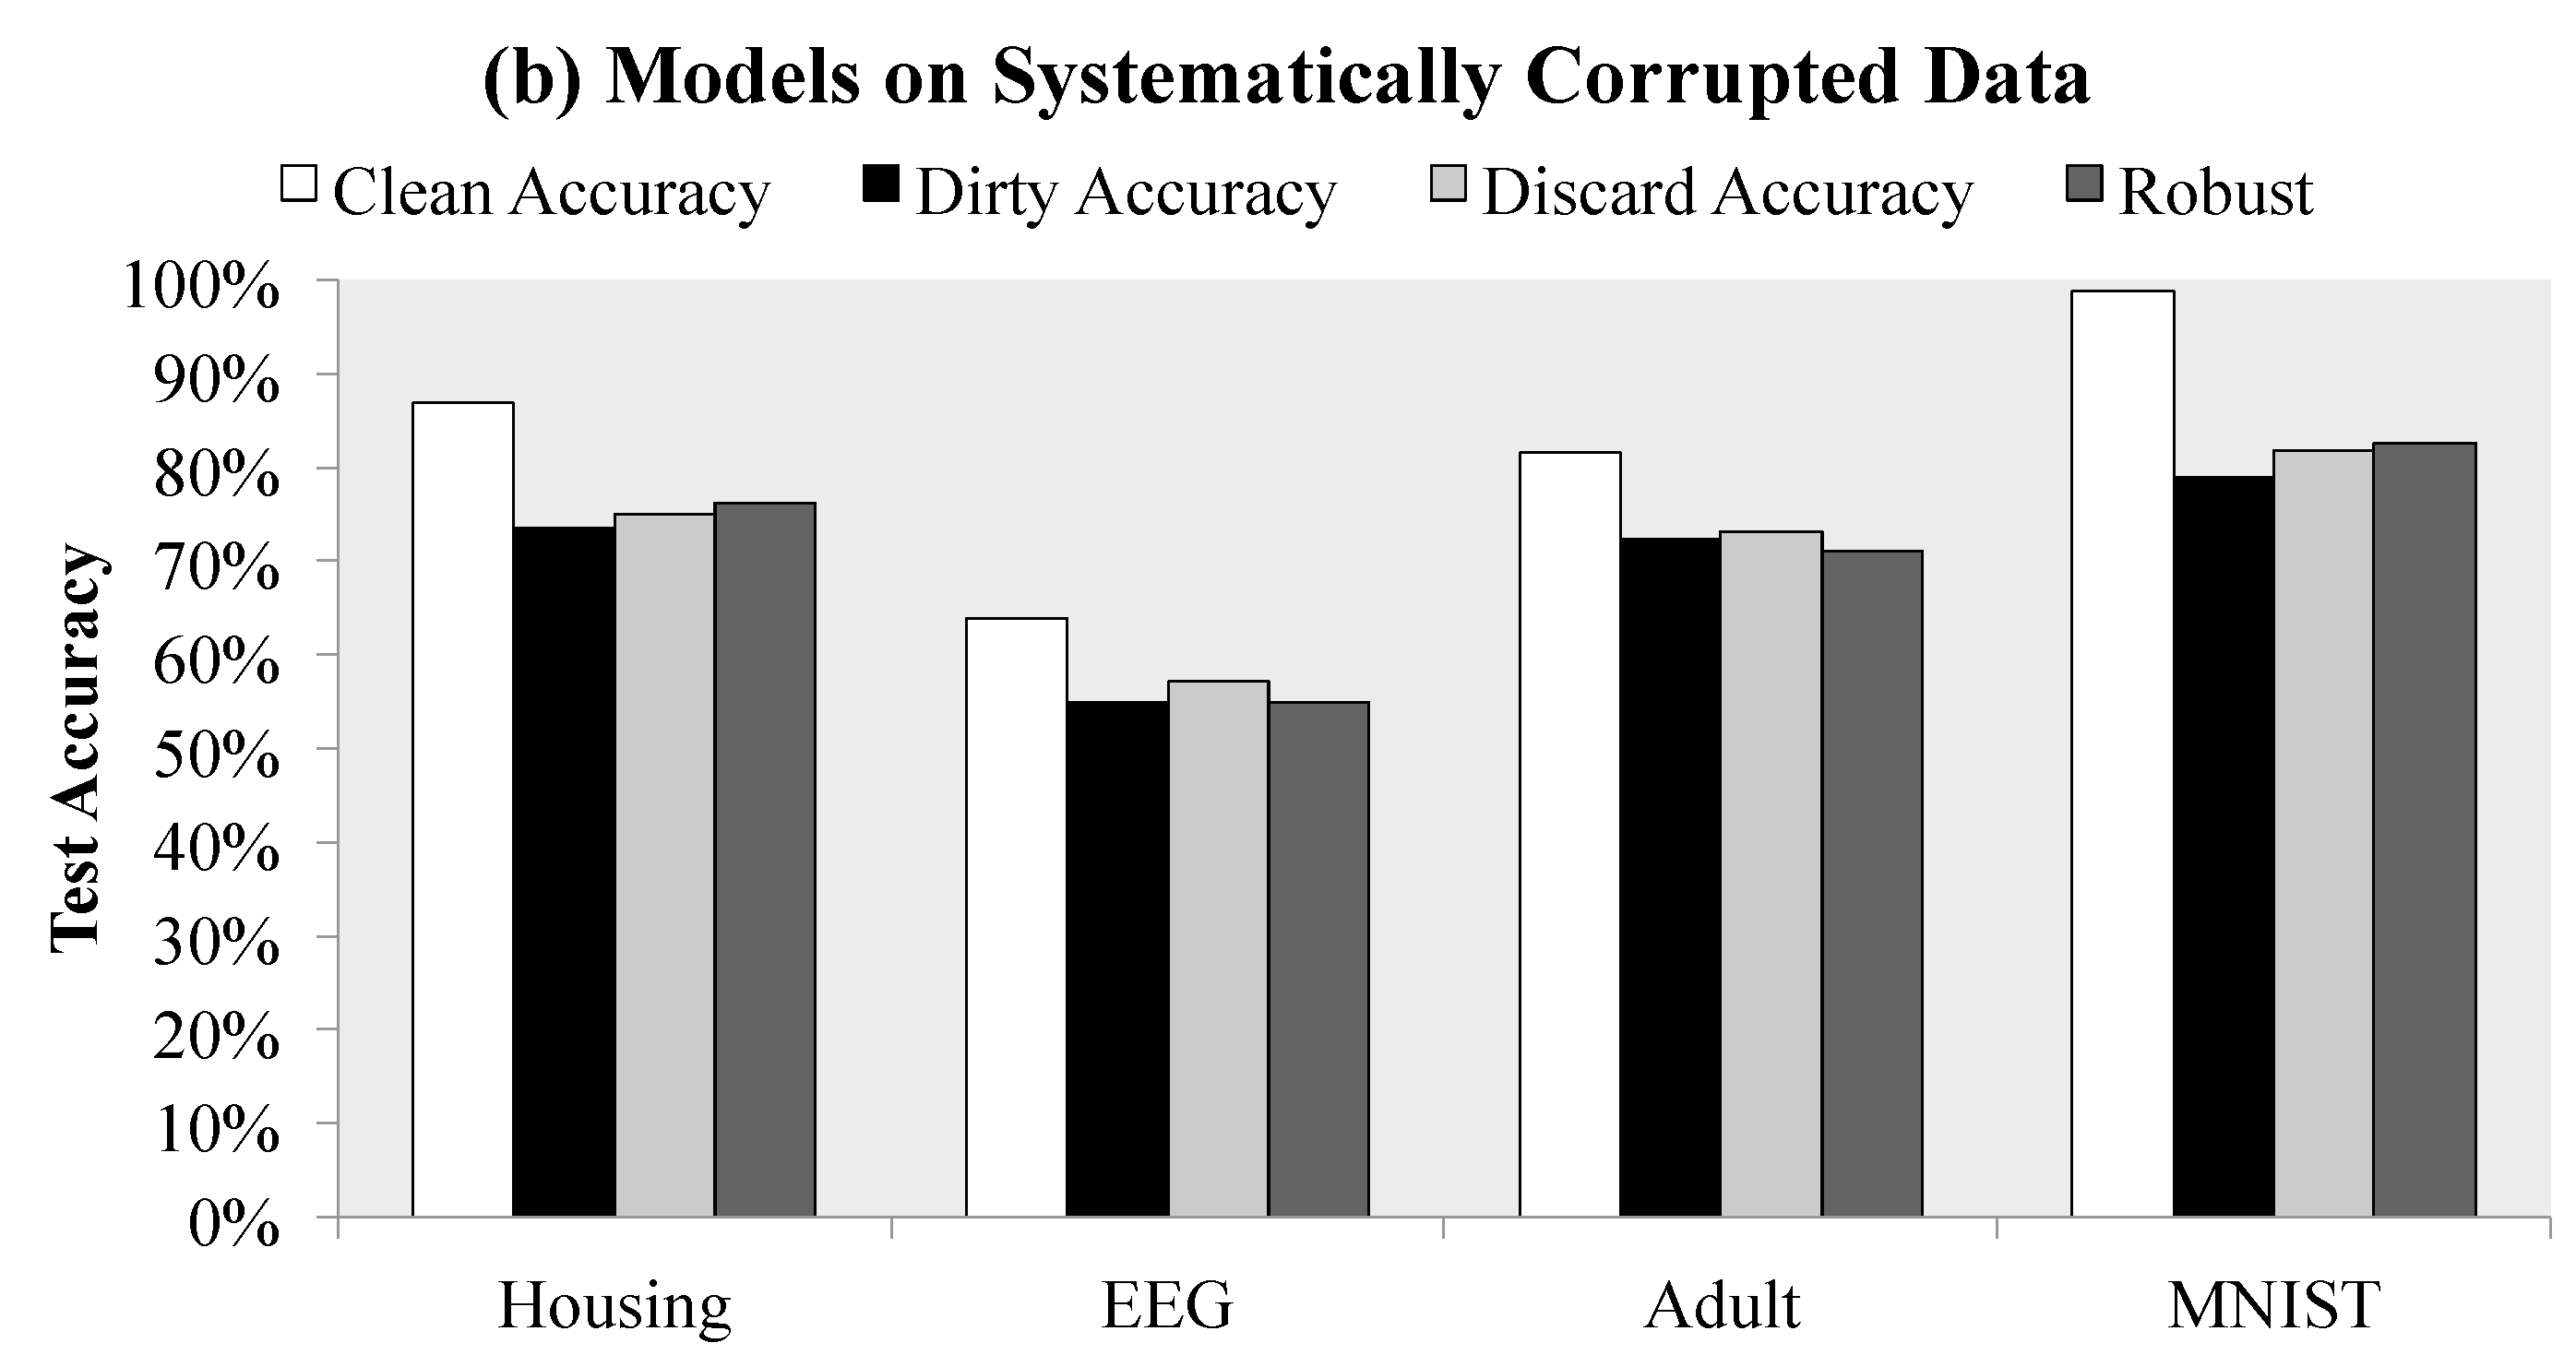
\includegraphics[width=0.49\columnwidth]{exp/exp1.pdf}
 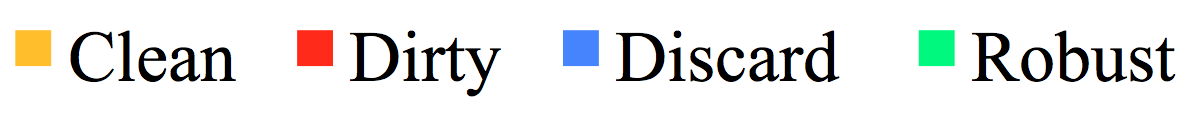
\includegraphics[width=0.5\columnwidth]{exp/legend-1.png}
 \caption{(a) Robust techniques and discarding data work when corrupted data are random and look atypical. (b) Data cleaning can provide reliable performance in both the systematically corrupted setting and randomly corrupted setting.\label{sys-rand}}
\end{figure}

\subsubsection{Data Cleaning v.s. Robust Statistics}
Machine Learning has broadly studied a number of \emph{robust} methods to deal with some types of outliers. In particular, this field studies random high-magnitude outliers and techniques to make statistical model training agnostic to their presence. Feng et al. proposed a variant of logistic regression that is robust to outliers~\cite{feng2014robust}. We chose this algorithm because it is a robust extension of the convex regularized loss model, leading to a better apples-to-apples comparison between the techniques.
Our goal is to understand which types of data corruption are amenable to data cleaning and which are better suited for robust statistical techniques.
The experiment compares four schemes: (1) full data cleaning, (2) baseline of no cleaning, (3) discarding the dirty data, and (4) robust logistic regression. 
We corrupted 5\% of the training examples in each dataset in two different ways:

\vspace{0.5em}

\noindent\textbf{Random Corruption: } Simulated high-magnitude random outliers. 5\% of the examples are selected at random and a random feature is replaced with 3 times the highest feature value.

\vspace{0.5em}

\noindent\textbf{Systematic Corruption: } Simulated innocuous looking (but still incorrect) systematic corruption. The model is trained on the clean data, and the three most important features (highest weighted) are identified. The examples are sorted by each of these features and the top examples are corrupted with the mean value for that feature (5\% corruption in all). 
%It is important to note that examples can have multiple corrupted features.

Figure \ref{sys-rand} shows the test accuracy for models trained on both types of data with the different techniques.
The robust method performs well on the random high-magnitude outliers with only a 2.0\% reduction in clean test accuracy for EEG and 2.5\% reduction for Adult.
In the random setting, discarding dirty data also performs relatively well.
However, the robust method falters on the systematic corruption with a 9.1\% reduction in clean test accuracy for EEG and 10.5\% reduction for Adult.
%Data cleaning is the most reliable option across datasets and corruption types.
The problem is that without cleaning, there is no way to know if the corruption is random or systematic and when to trust a robust method.
While data cleaning requires more effort, it provides benefits in both settings.
In the remaining experiments, unless otherwise noted, the experiments use systematic corruption.

\iffalse
\begin{figure}[t]
\centering\vspace{-1em}
 %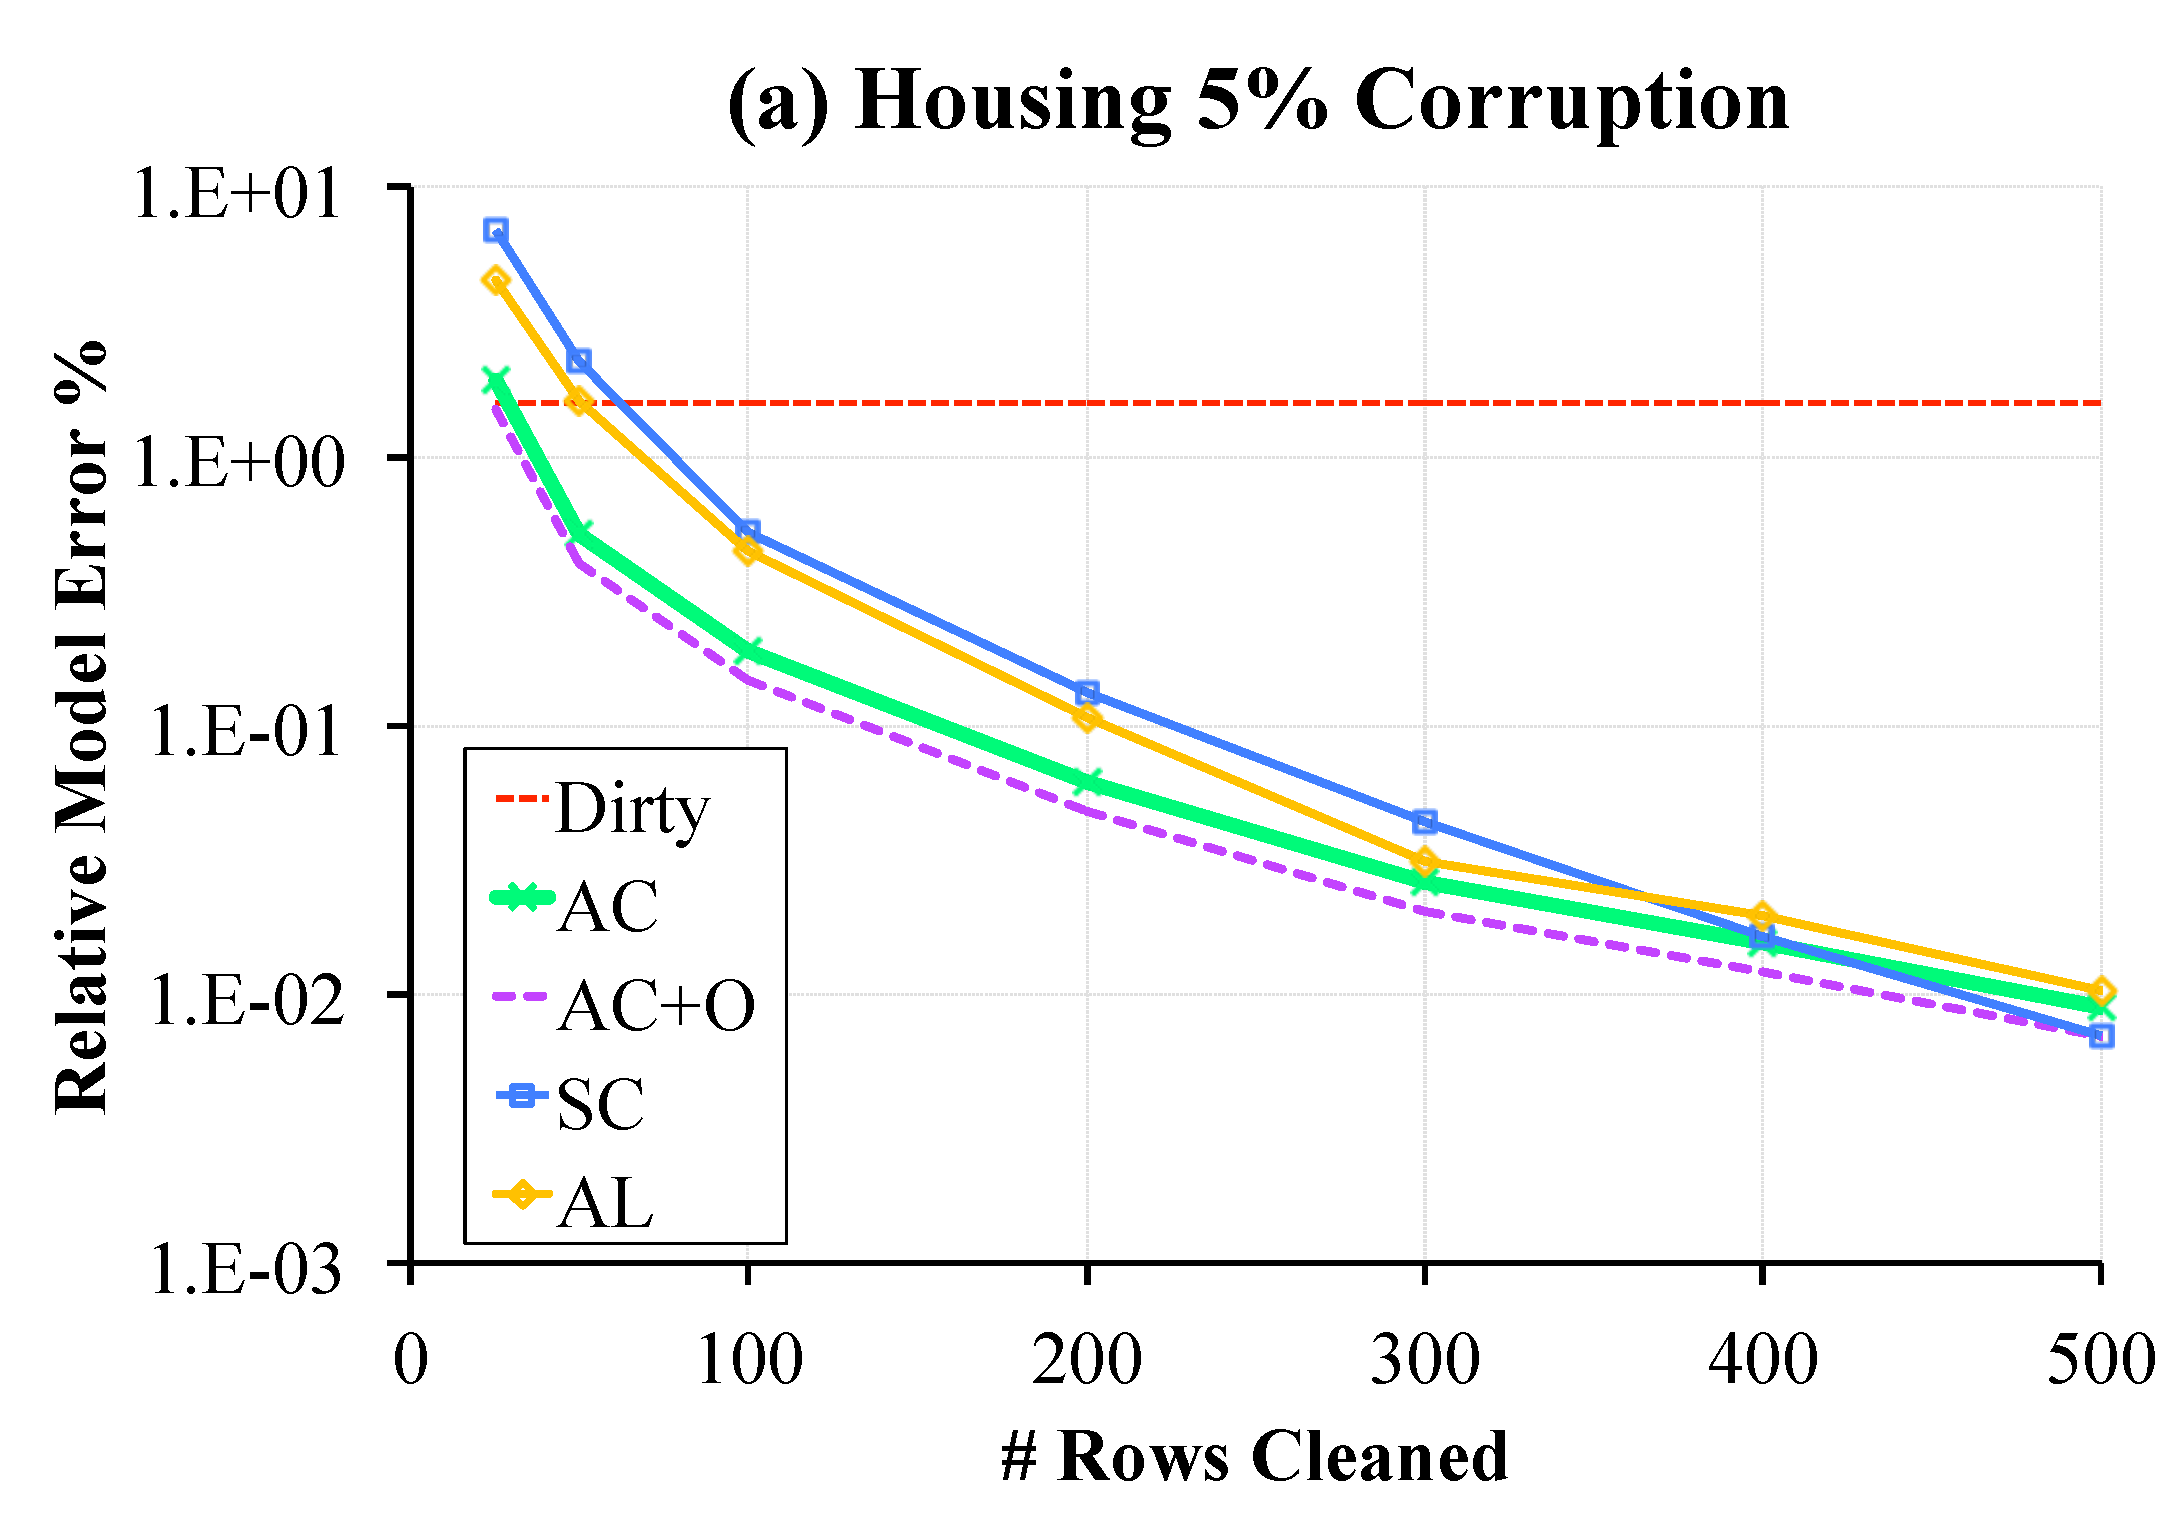
\includegraphics[scale=0.15]{exp/exp3a.pdf}
 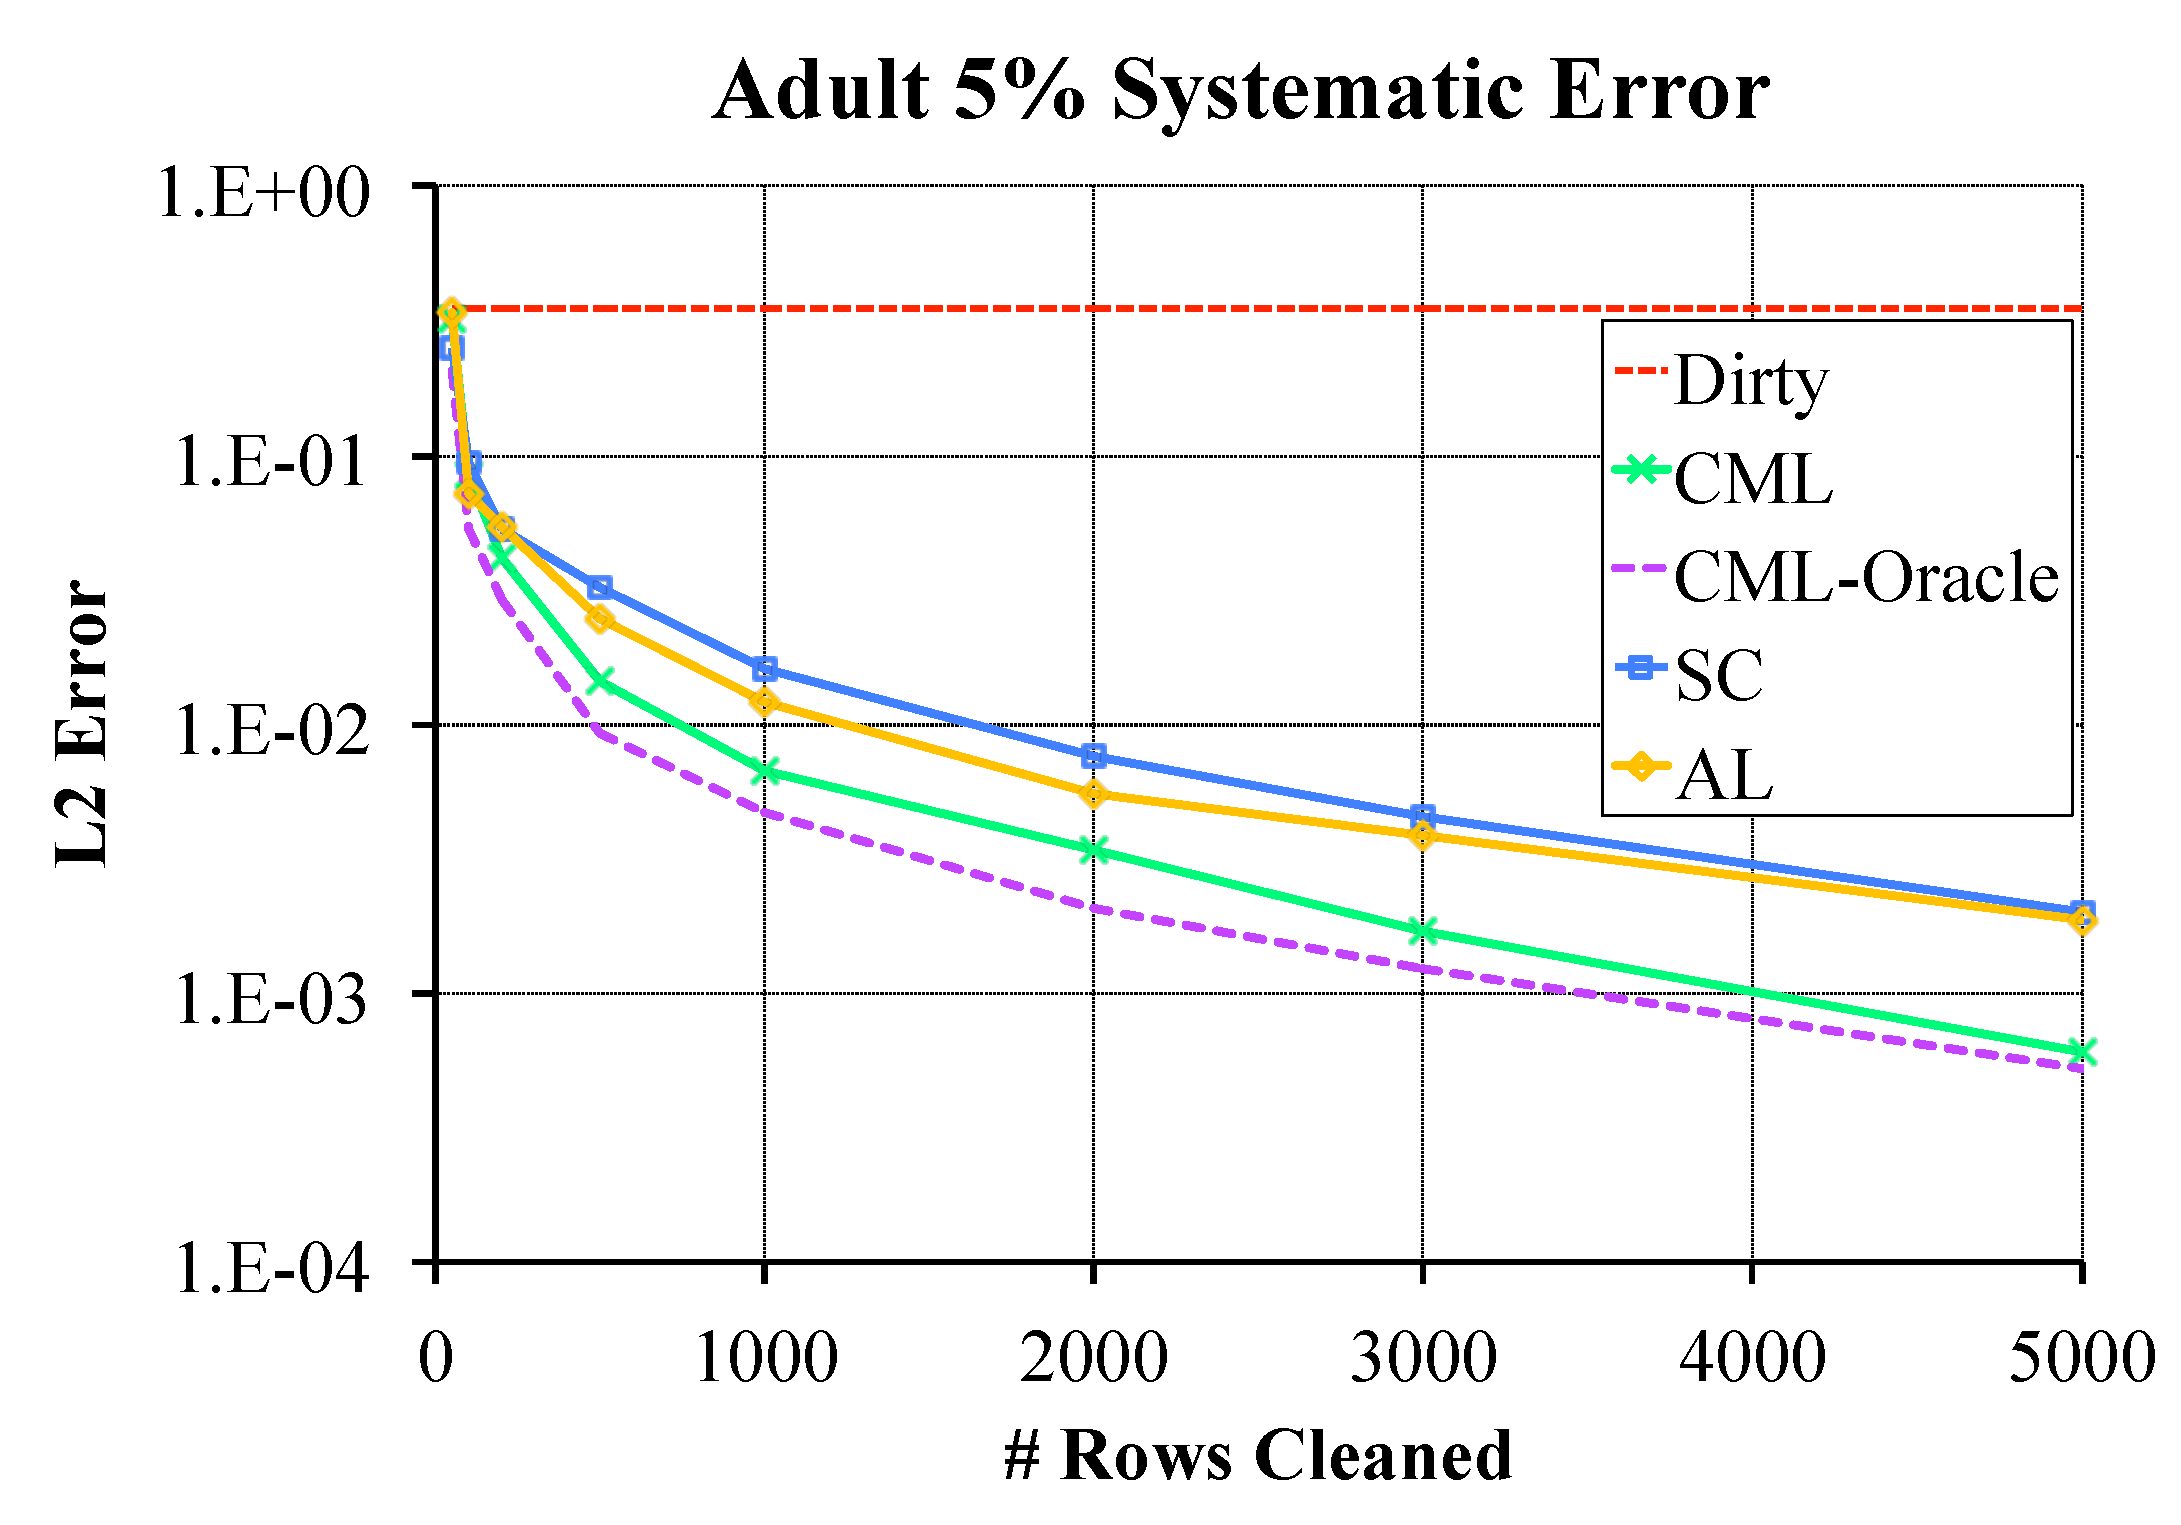
\includegraphics[width=0.49\columnwidth]{exp/exp3b.pdf}
  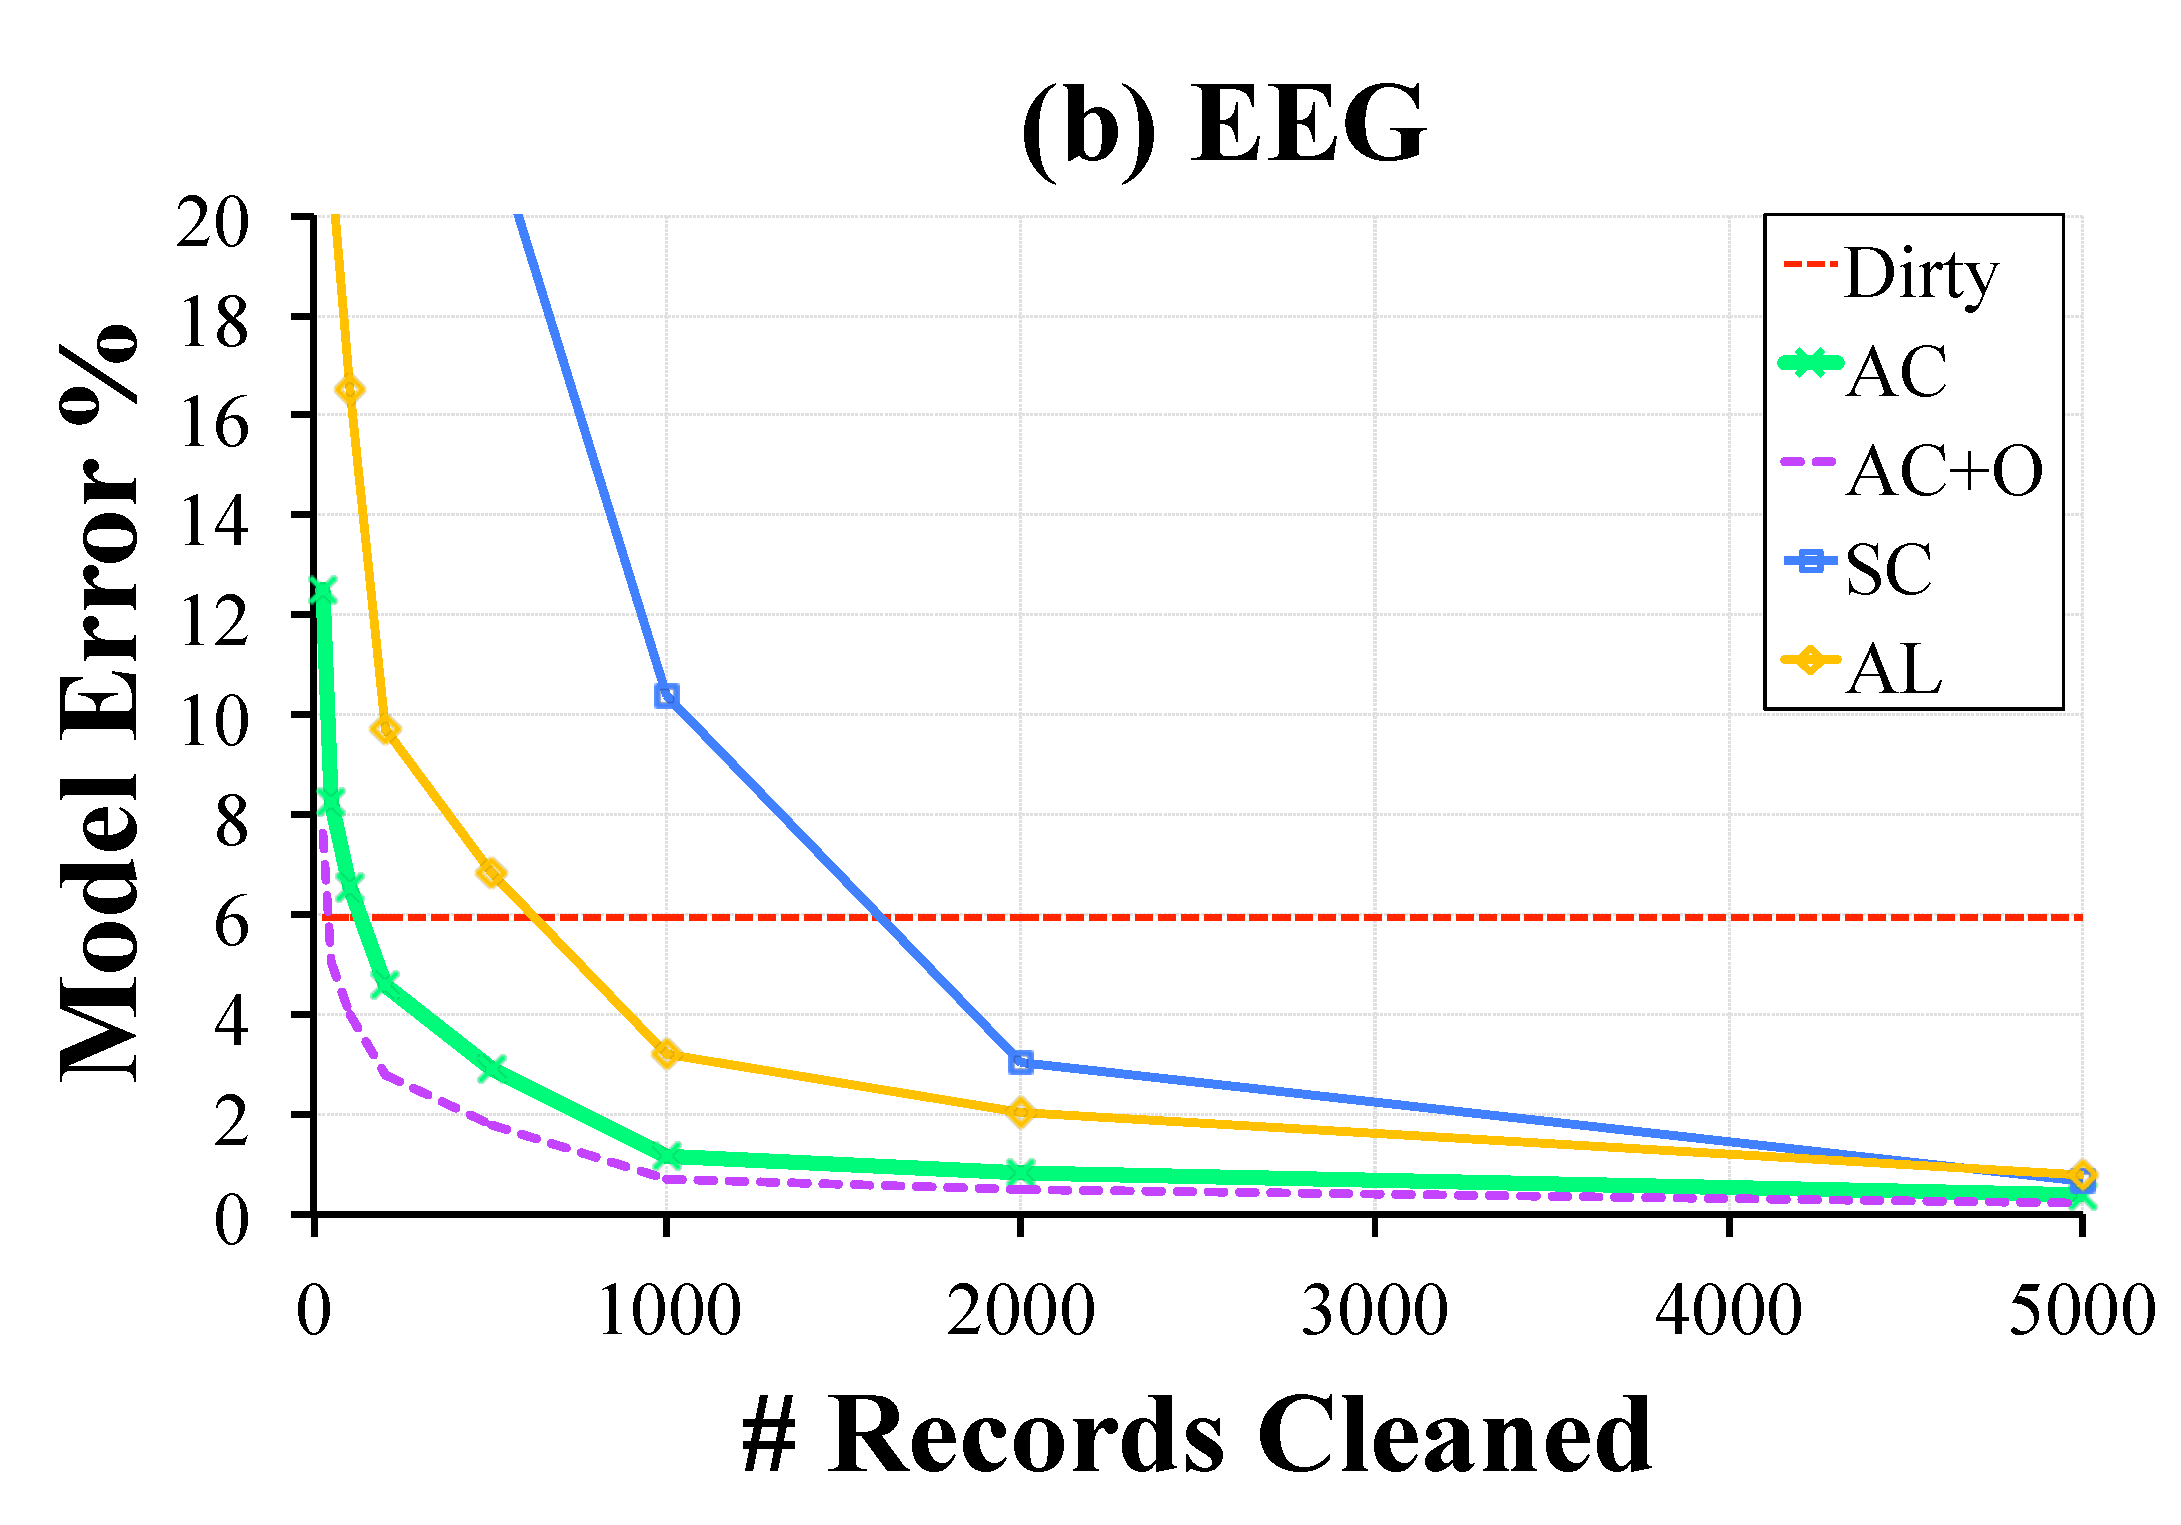
\includegraphics[width=0.49\columnwidth]{exp/exp3c.pdf}
  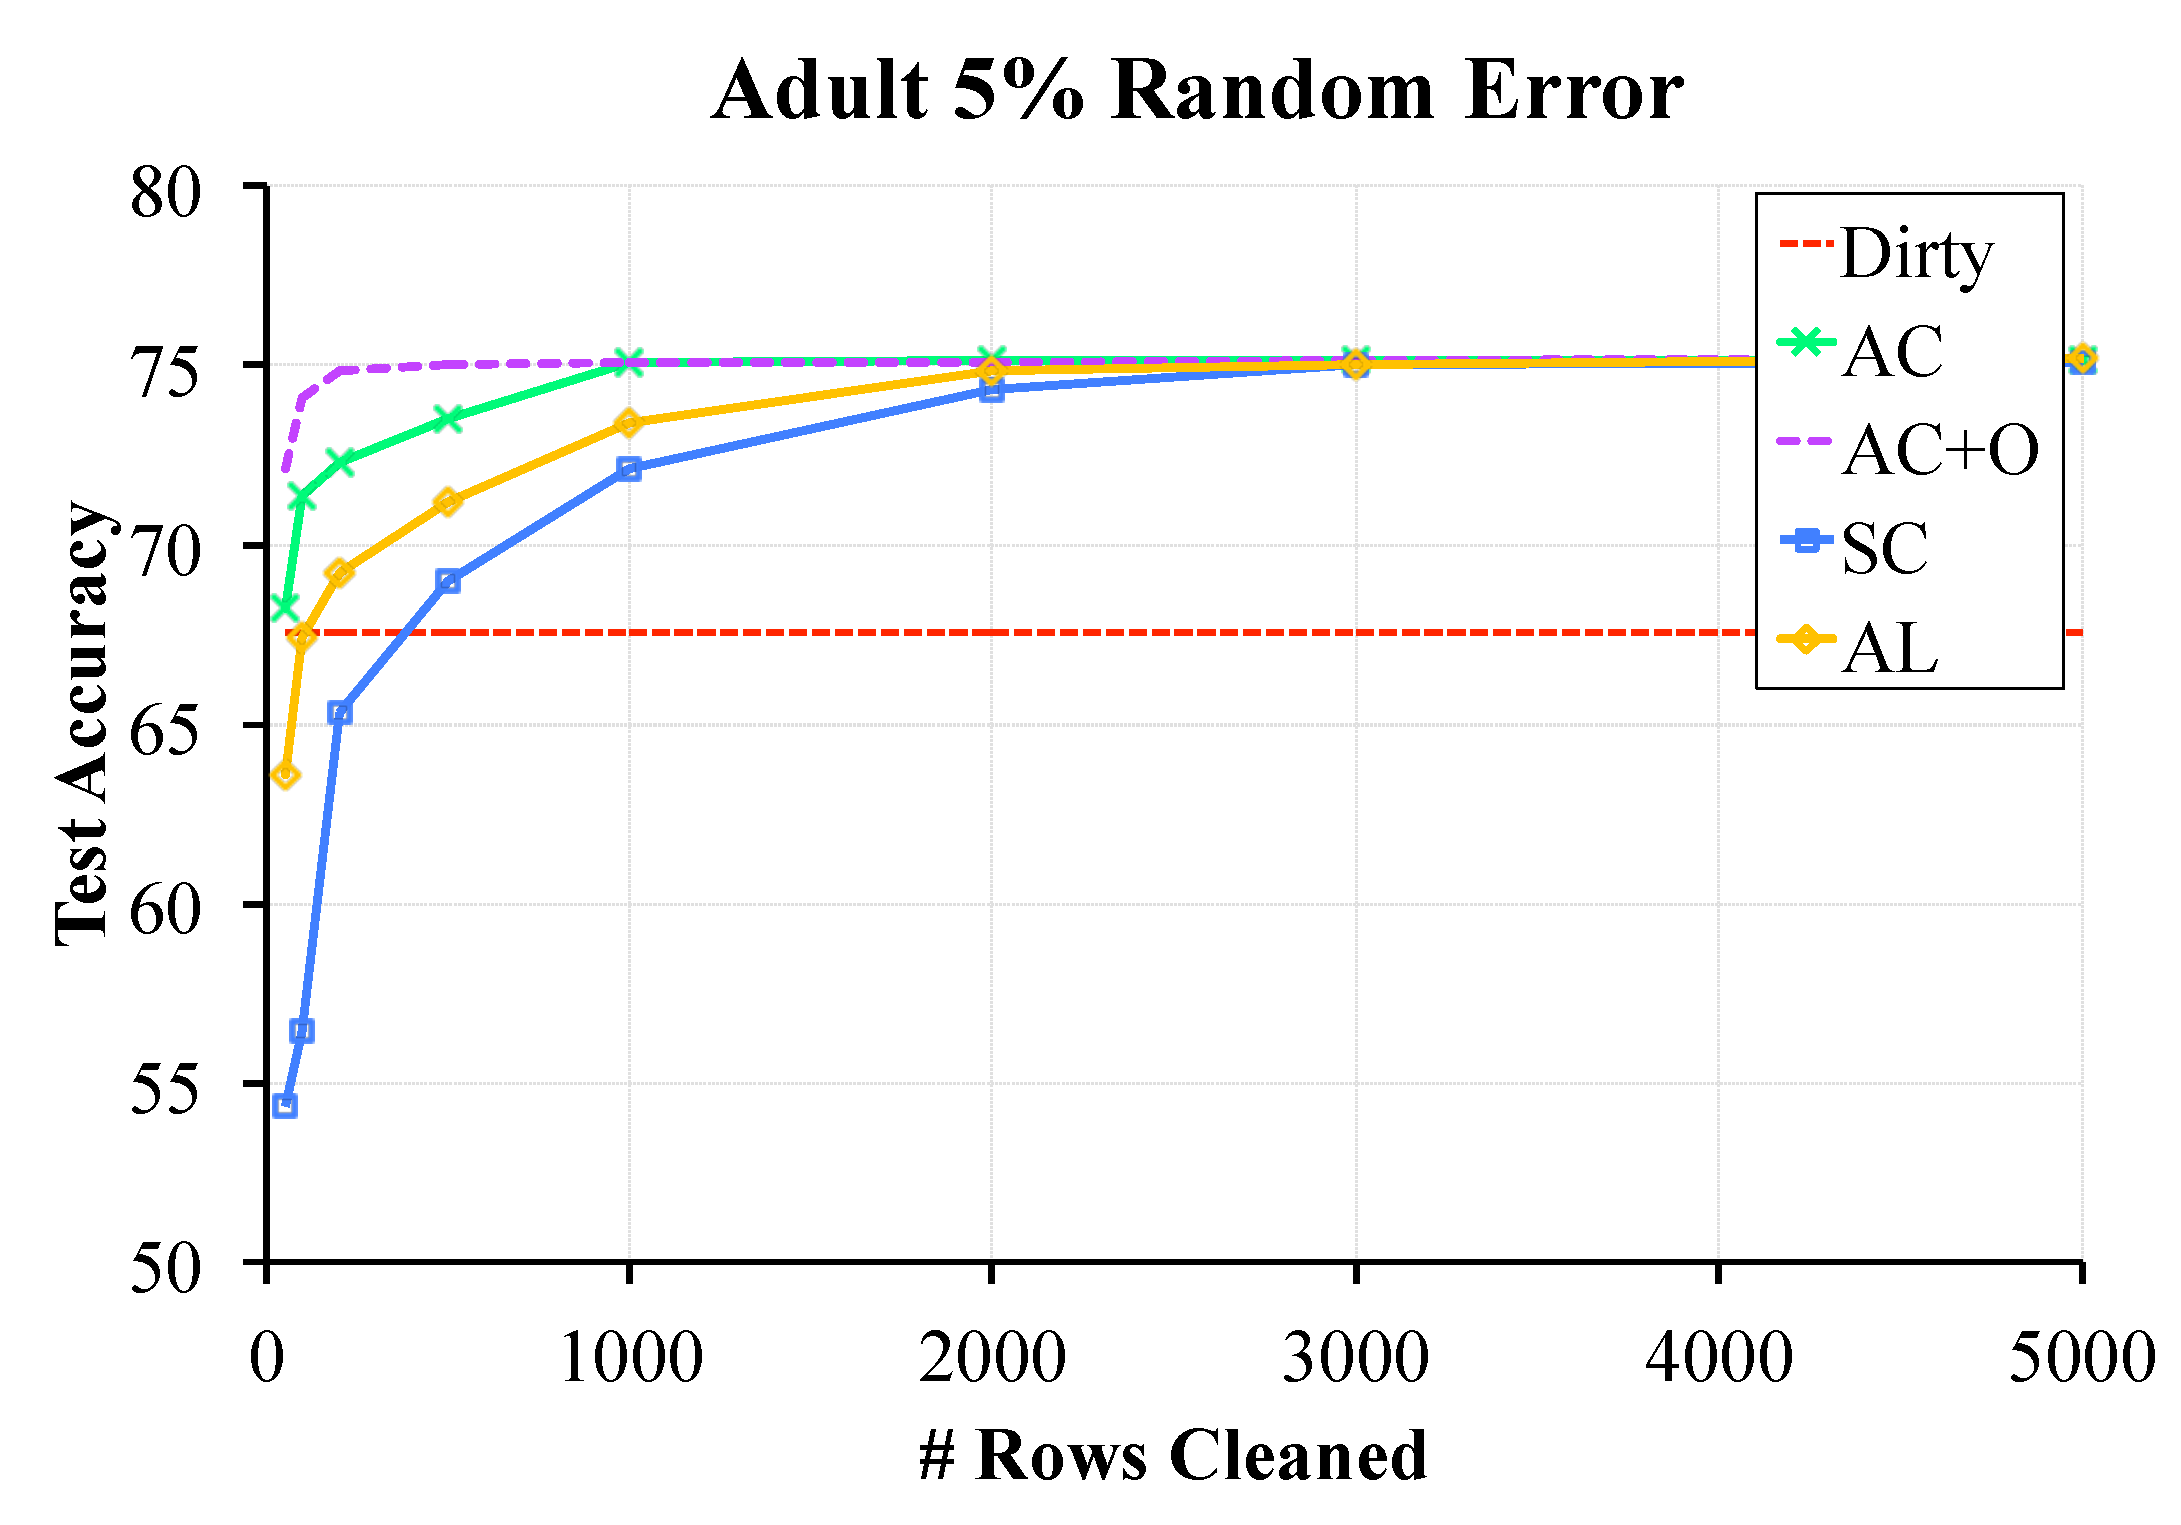
\includegraphics[width=0.49\columnwidth]{exp/exp3bb.pdf}
  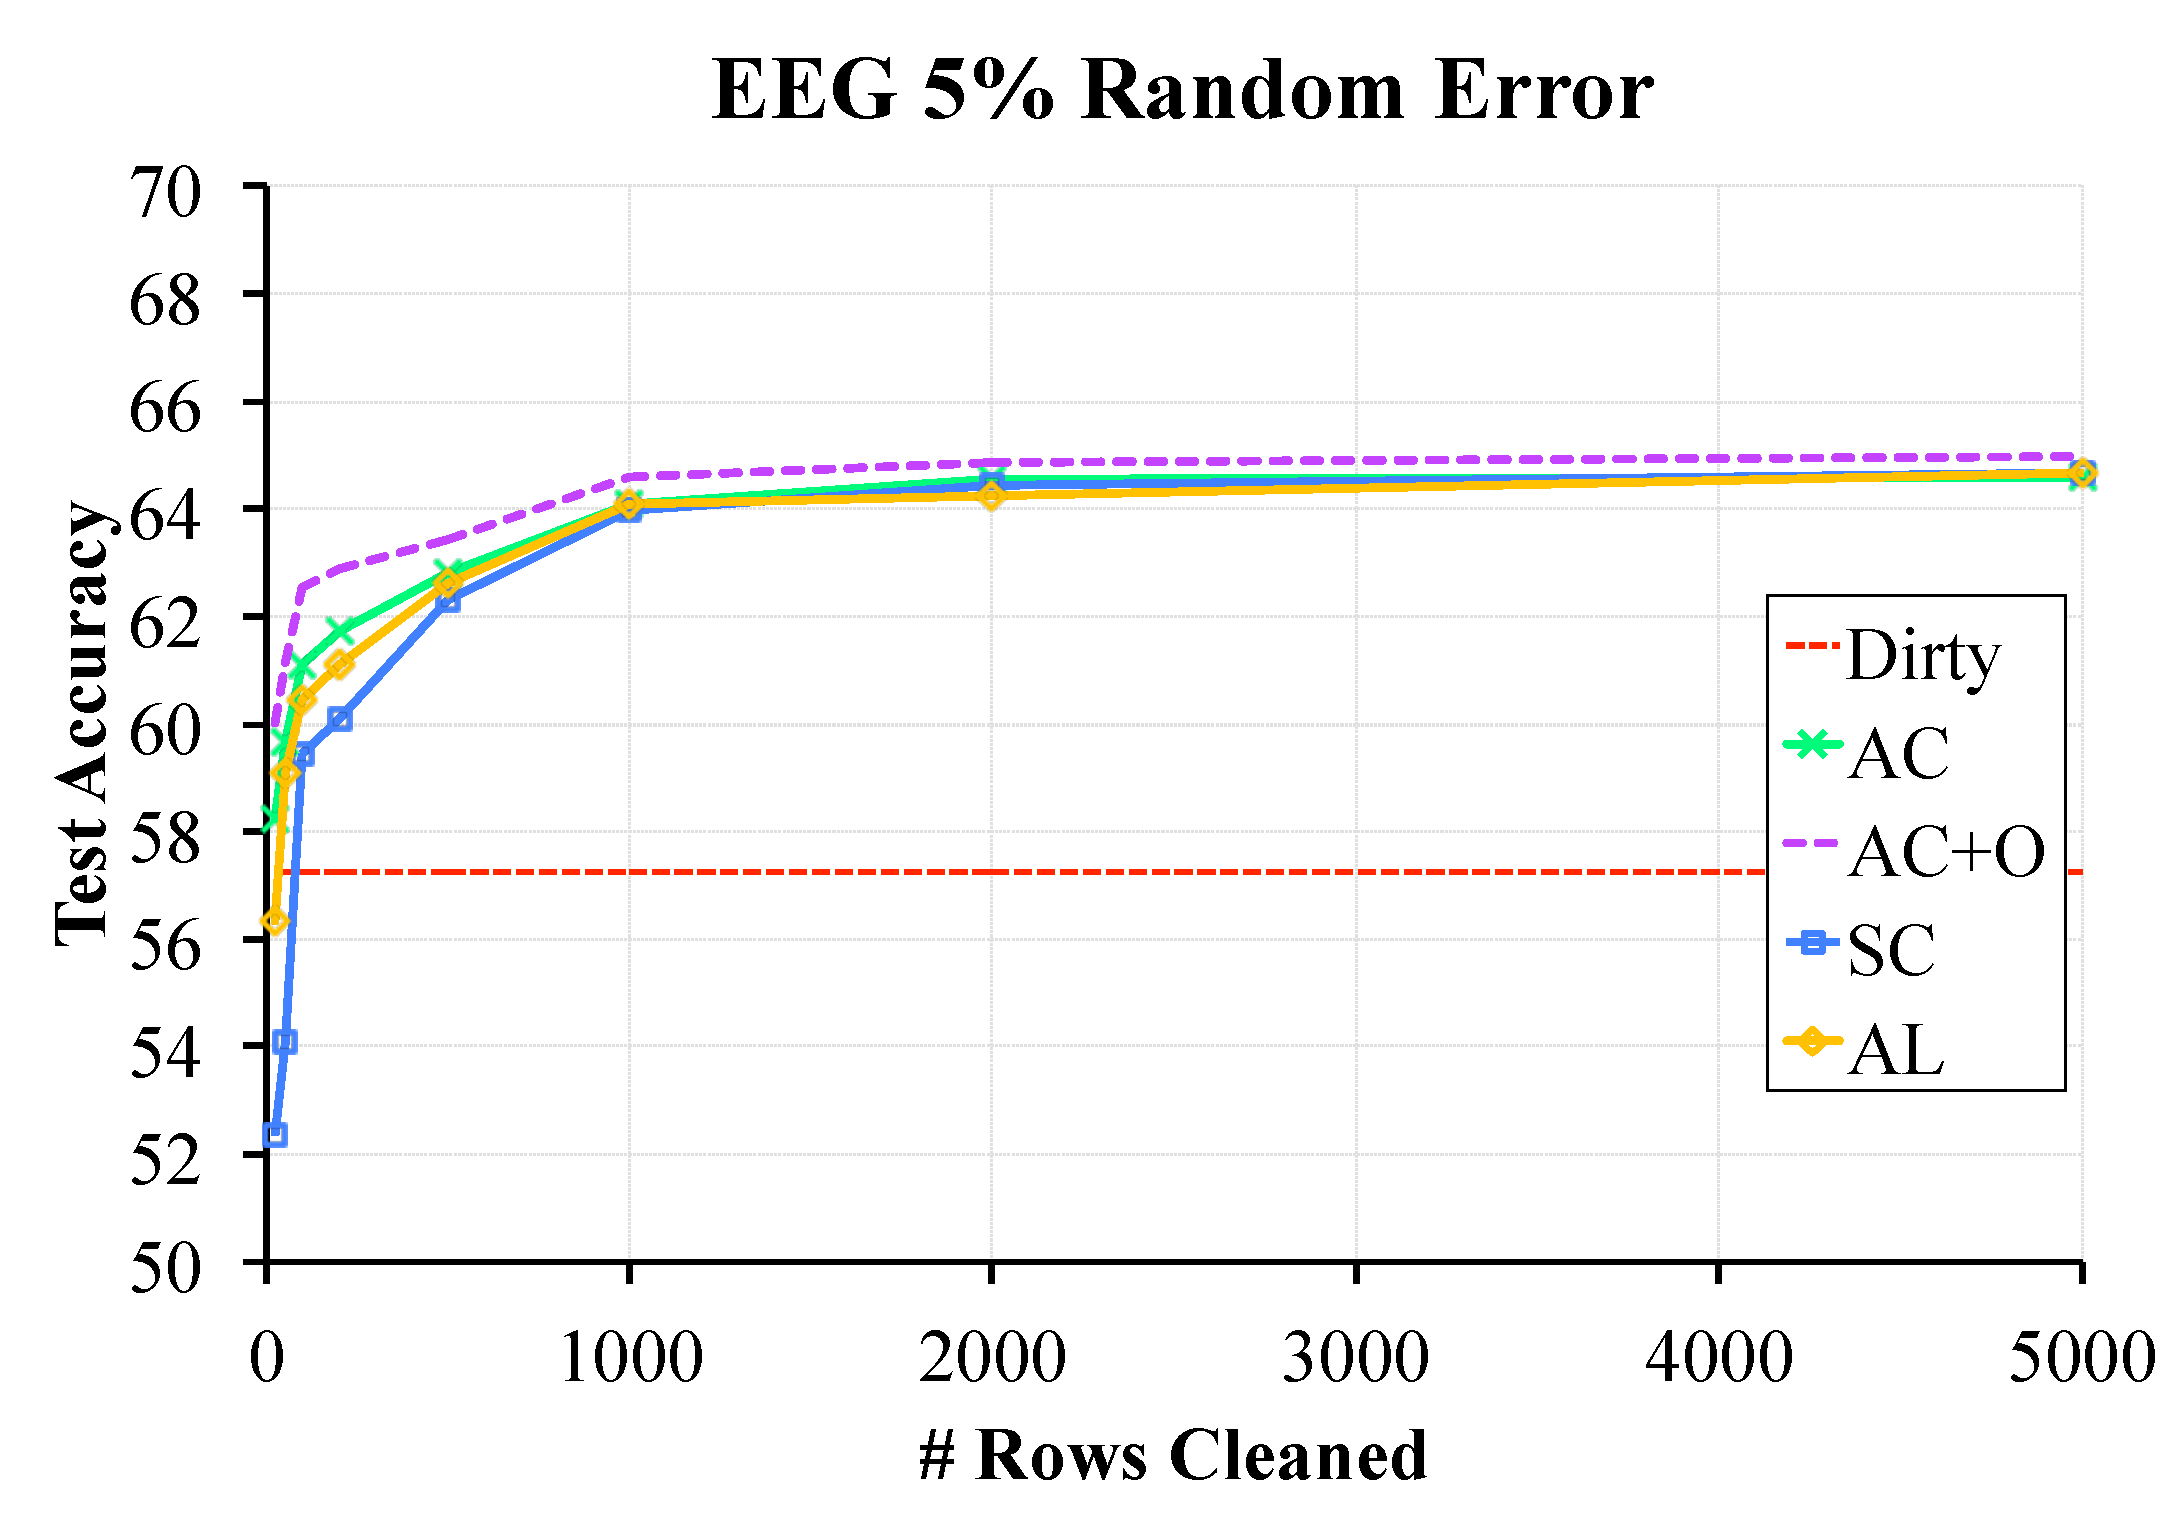
\includegraphics[width=0.49\columnwidth]{exp/exp3cc.pdf}
  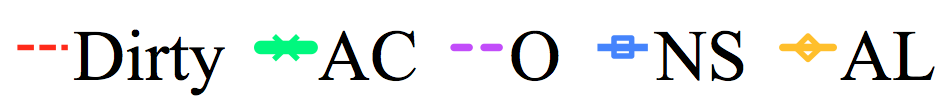
\includegraphics[width=0.5\columnwidth]{exp/legend-general.png}\vspace{-0.5em}
 \caption{ The relative model error as a function of the number of examples cleaned. \sys converges with a smaller sample size to the true result in comparison to Active Learning and Naive-Sampling. \label{prio-perf}}\vspace{-1em}
\end{figure}

\subsubsection{Samples-to-Error}
This experiment evaluates the samples-to-error tradeoff between four alternative algorithms: \sys (AC), SampleClean, Active Learning, and \sys+Oracle (AC+O).
Figure \ref{prio-perf} shows the model error and test accuracy as a function of the number of cleaned records.
In terms of model error, \sys gives its largest benefits for small sample sizes.
For 500 cleaned records of the Adult dataset, \sys has 6.1x less error than SampleClean and 2.1x less error than Active Learning.
For 500 cleaned records of the EEG dataset, \sys has 9.6x less error than SampleClean and 2.4x less error than Active Learning.
Both Active Learning and \sys benefit from the initialization with the dirty model as they do not retrain their models from scratch, and \sys improves on this performance with detection and error estimation.
Active Learning has no notion of dirty and clean data, and therefore prioritizes its selections with respect to the dirty data.
These gains in model error also correlate well to improvements in test error (defined as the test accuracy difference w.r.t cleaning all data).
The test error converges more quickly than model error, emphasizing the benefits of progressive data cleaning since it is not necessary to clean all the data to get a model with essentially the same performance as the clean model.
For example, to achieve a test error of 1\% on the Adult dataset, \sys cleans 500 fewer records than Active Learning.
\fi

\subsubsection{Dirty Data Detection}
The adaptive detection depends on being able to predict corrupted records.
For example, random corruption not correlated with any other data features may be hard to learn.
As corruption becomes more random, the classifier becomes increasingly erroneous.
This experiment explores making the systematic corruption more random.
Instead of selecting the highest valued records for the most valuable features, we corrupt random records with probability $p$. 
We compare these results to AC-D where we do not have a detector at all at one vertical slice of the previous plot (cleaning 1000 records).
Figure \ref{tradeoffs2}a plots the relative error reduction using a classifier.
When the corruption is about 50\% random then there is a break even point where no detection is better.
The classifier is imperfect and misclassifies some data points incorrectly as cleaned.

\begin{figure}[ht!]
\centering
 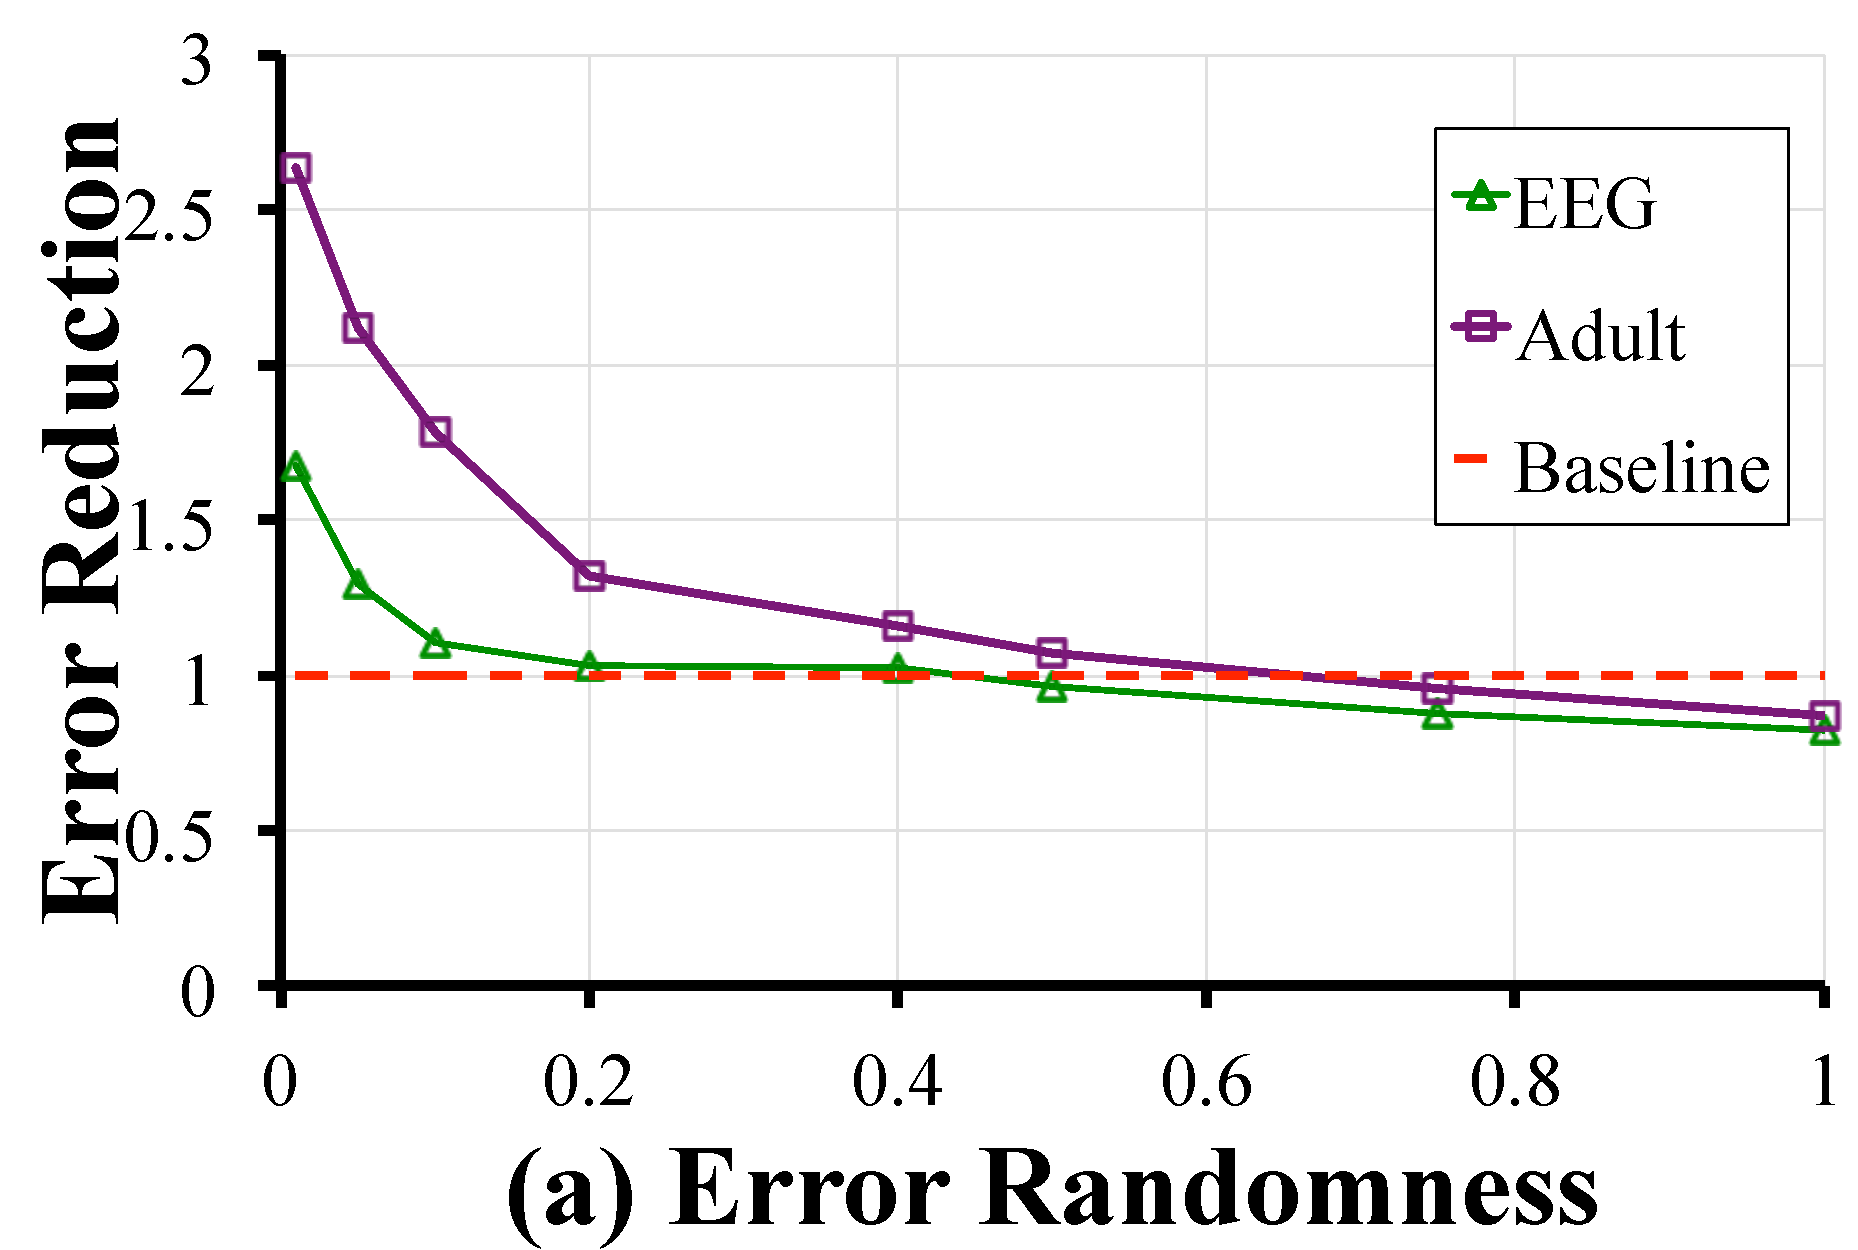
\includegraphics[width=0.49\columnwidth]{exp/exp5a.pdf}
 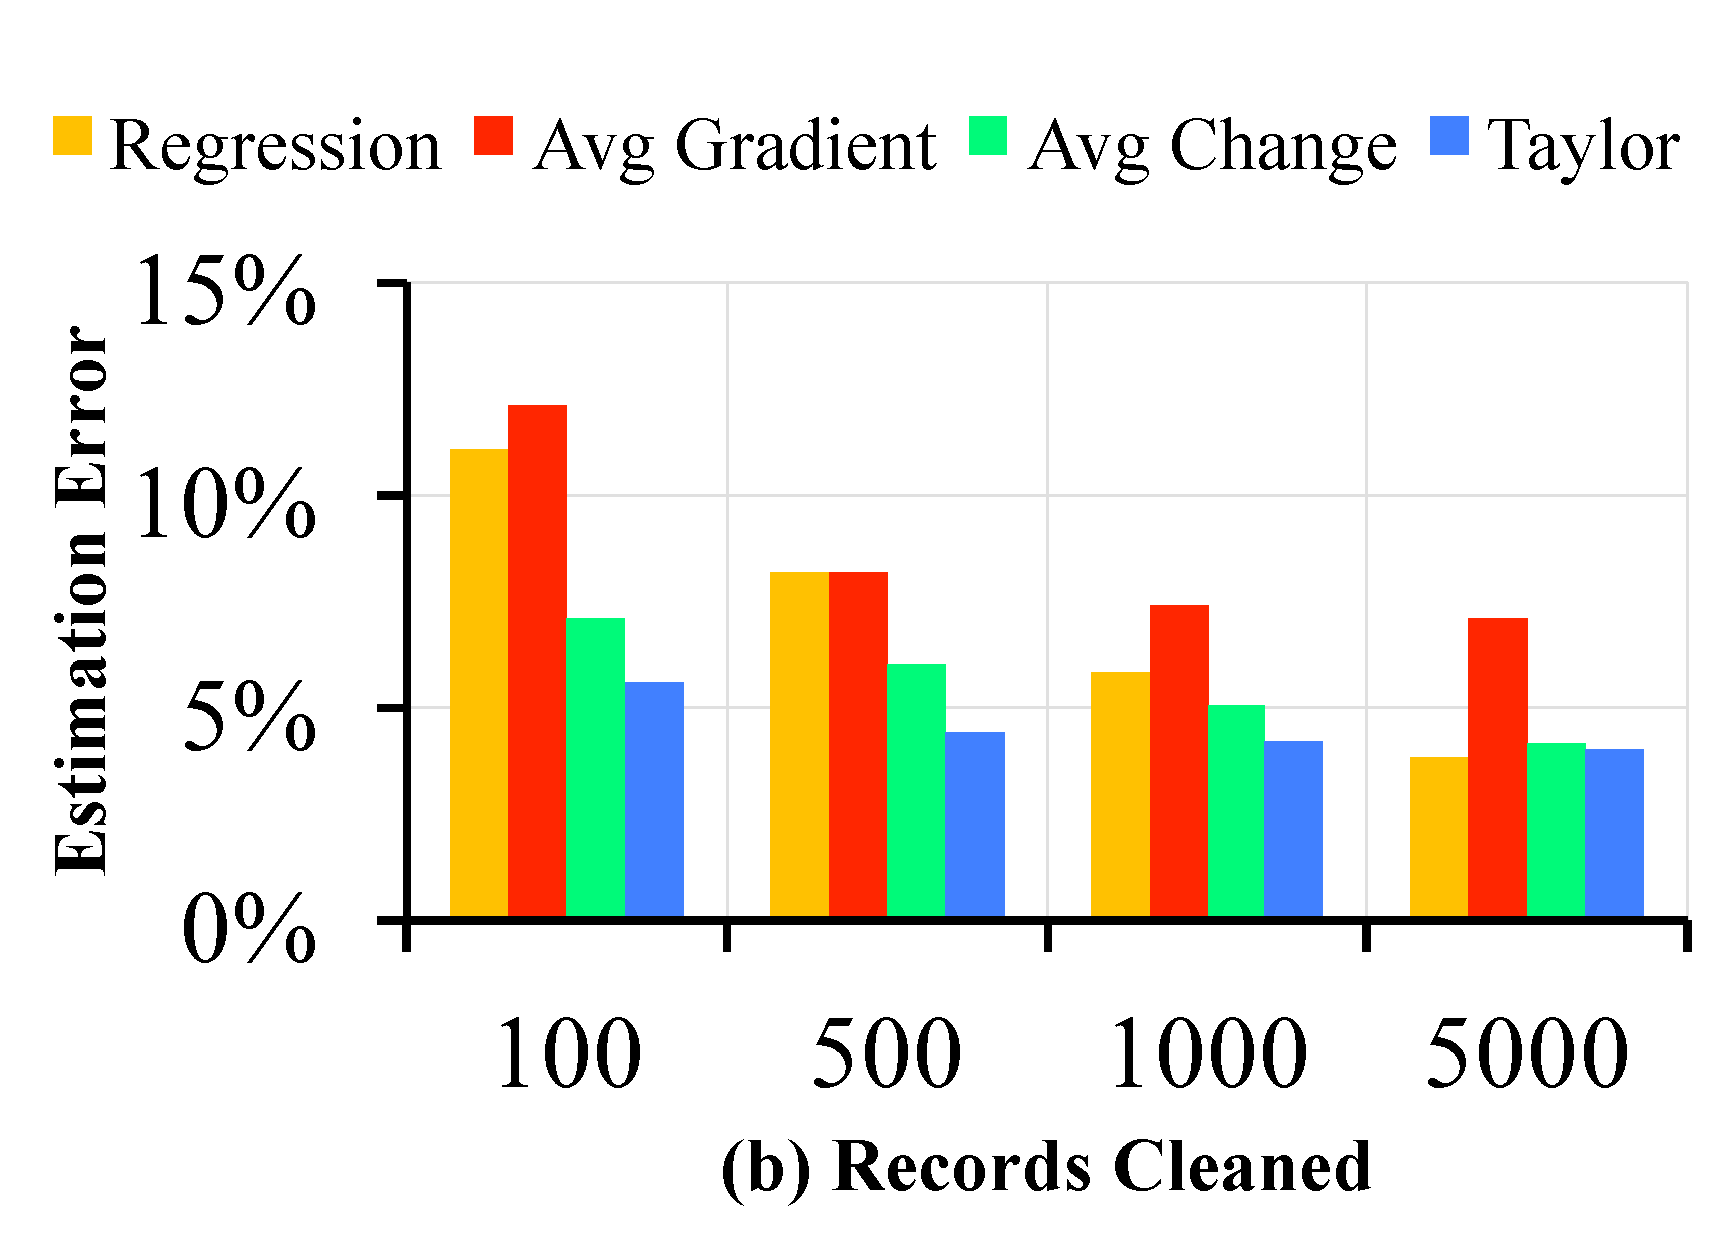
\includegraphics[width=0.49\columnwidth]{exp/exp12.pdf}\vspace{-0.5em}
 \caption{(a) Data corruptions that are less random are easier to classify, and lead to more significant reductions in relative model error. (b) The Taylor series approximation gives more accurate estimates when the amount of cleaned data is small. \label{tradeoffs2}}
\end{figure}

\subsubsection{Impact Estimation}\label{est}
This experiment compares estimation techniques: (1) ``linear regression" trains a linear regression model that predicts the clean gradient as a function of the dirty gradient, (2) ``average gradient" which does not use the detection to inform how to apply the estimate, (3) ``average feature change" uses detection but no linearization, and (4) the Taylor series linear approximation.
Figure \ref{tradeoffs2}b measures how accurately each estimation technique estimates the gradient as a function of the number of examined records on the EEG dataset.
Estimation error is measured using the relative L2 error with the true gradient.
The Taylor series approximation proposed gives more accurate for small cleaning sizes.
Linear regression and the average feature change technique do eventually perform comparably but only after cleaning much more data.
